\documentclass[11pt]{article}
\usepackage[margin=1in]{geometry}
\usepackage{amsmath,booktabs,array,hyperref}
\usepackage{pgfplots}
\usepgfplotslibrary{groupplots}
\pgfplotsset{compat=1.18}
\definecolor{papercolor}{RGB}{100,116,139}
\definecolor{repcolor}{RGB}{124,58,237}
\definecolor{lstmcolor}{RGB}{37,99,235}
\definecolor{transcolor}{RGB}{234,88,12}
\definecolor{blendcolor}{RGB}{22,163,74}
\hypersetup{colorlinks=true,urlcolor=blue,linkcolor=blue}
\title{Extending Deep Learning in Asset Pricing:\\Architecture, Rolling Performance, and Economic Regimes}
\author{Reza Zamani\\Research draft based on saved replication experiments}
\date{October 5, 2026}
\begin{document}
\maketitle
\begin{abstract}
This study extends an existing asset-pricing replication by comparing LSTM and causal Transformer macroeconomic encoders under a common reduced training budget. It evaluates fixed portfolio returns over rolling windows, economic regimes, and their combination. Eighteen models, nine per architecture, are trained using a shortened three-stage schedule. Over the 1992--2016 test period, monthly Sharpe is 0.459 for LSTM and 0.304 for Transformer. Average annualized rolling Sharpe also favors LSTM at both 36 and 60 months. Conditional-month regime analysis favors LSTM in expansion, recession, high-volatility, and low-volatility groups. However, trailing windows classified by their endpoint regime answer a different question and reveal a small Transformer advantage for 36-month windows ending in recessions. A fixed equal-weight return blend achieves monthly test Sharpe of 0.463. These are descriptive findings under a restricted optimization budget, not evidence that one architecture universally dominates or that published results have been exactly reproduced.
\end{abstract}
\section{Research question and contribution}
Chen, Pelger, and Zhu's framework combines an economic pricing objective, adversarial instruments, and an LSTM representation of macroeconomic dynamics \cite{cpz}. Our study asks whether replacing the recurrent macroeconomic encoders with causal attention changes the performance of the replicated pricing-factor portfolios.

The first addition is a matched-budget architecture experiment: both the SDF and instrument macroeconomic encoders are replaced while their output dimensions and the economic objective are retained. The second addition is a temporal comparison of those saved models over 36- and 60-month windows. The third is a conditional comparison across recession/expansion and market-volatility groups. The fourth combines the temporal and economic views by classifying rolling windows according to the state at their ending month. A fixed 50/50 return blend provides a separate diversification illustration.

These additions are the scope of this replication extension. We do not establish priority over other research, introduce a new pricing restriction, or treat evaluation windows and regime labels as new trained models. In particular, rolling evaluation does not imply rolling retraining.

\subsection{Comparison design: what is replicated and what is added?}
We separate three evidentiary layers. First, the published results establish the benchmark. Second, Code 07 measures how our historical replication compares with that benchmark. Third, Codes 08--11 introduce an architectural comparison and a structured evaluation of its saved results. Maintaining these layers prevents a reduced-budget experiment from being presented as the original paper's implementation.
\begin{table}[htbp]\centering\small
\caption{Contribution map and the question answered by each comparison.}\label{tab:contributions}
\begin{tabular}{p{.18\linewidth}p{.36\linewidth}p{.36\linewidth}}\toprule
Layer & Comparison & Research question \\\midrule
Replication & Paper LS/EN/FFN/GAN versus Code 07 & How closely do we reproduce the original ordering and Sharpe? \\
Architecture & New LSTM versus causal Transformer & Does replacing the macro encoder help at the same optimization budget? \\
Time variation & Fixed-model 36/60-month rolling returns & When is each architecture relatively stronger? \\
Economic states & Labeled recession/volatility months & In which states do return and risk differ? \\
Combined view & Rolling statistics by endpoint state & How does trailing relative performance vary with economic endpoints? \\
Diversification & Fixed 50/50 return blend & Does simple averaging change the return/risk trade-off? \\\bottomrule
\end{tabular}\end{table}

\section{Data, model specification, and estimation}
The local panel uses 46 firm characteristics and 178 macroeconomic inputs with chronological splits: January 1967--December 1986 for training (240 months), January 1987--December 1991 for validation (60 months), and January 1992--December 2016 for testing (300 months). Existing preprocessing and masks for inactive observations are retained. Test results were examined in preceding exploratory work, so the report is not a newly sealed holdout evaluation.

The pricing-weight network has two 64-unit hidden layers and a four-dimensional macroeconomic state. The conditional instrument network uses a 32-dimensional state and eight bounded instruments. The Transformer uses model dimension 32, four attention heads, two layers, feedforward dimension 64, positional encoding, and a causal mask. State projections retain the required four and 32 dimensions. Both architectures use dropout 0.05 and Adam learning rate 0.001. Causal perturbation and prefix checks confirm that future macro inputs do not change earlier states; the macroeconomic data themselves are not a real-time-vintage dataset.

We preserve the audited author-style weighted moment objective, bounded instruments, validation checkpoint criteria, and raw-weight ensemble construction in a PyTorch implementation. Training has unconditional SDF, adversary, and conditional SDF stages. Runtime constraints shorten the schedule to 16, 4, and 48 epochs, respectively, with four optimizer passes and a four-epoch checkpoint warm-up. The audited author implementation instead uses 256, 64, and 1024 with a default warm-up of 64 \cite{code}. Our experiment is therefore a reduced-schedule port, not an exact implementation replication or a reproduction of the complete hyperparameter search.

Nine seeds (42--50) are run per architecture. Stage one selects the lowest validation unconditional loss; the final SDF stage selects the highest validation raw-factor Sharpe after warm-up. Adversary selection follows the audited training-loss convention. Selection is not based on test Sharpe. The eighteen models completed in approximately 12.9 minutes on the local CPU.

Within each architecture, raw stock weights are averaged across members and then normalized to monthly unit gross exposure. Ensemble Sharpe is computed from the resulting factor returns, not from the mean of member Sharpes. Our economic portfolio sign convention is consistent with expressing the SDF as one minus the weighted excess-return factor.
\section{Evaluation definitions}
For a return sample $\mathcal S$, monthly Sharpe is
\[
 SR_m(\mathcal S)=\frac{\bar r_{\mathcal S}}{\sqrt{|\mathcal S|^{-1}\sum_{t\in\mathcal S}(r_t-\bar r_{\mathcal S})^2}},\qquad SR_a=\sqrt{12}\,SR_m.
\]
The denominator uses population standard deviation. Annualization supplies a common display convention, rather than evidence that returns are independent. Means of rolling Sharpes are not equal to one full-period Sharpe because both the sample and the volatility denominator vary across windows.

Rolling Sharpe uses complete trailing windows of $W=36$ or $60$ test months. There are 265 and 241 complete windows, ending initially in December 1994 and December 1996. The trained models remain fixed throughout evaluation. All gross wealth calculations omit costs and use the inherited factor-return definition.

Business-cycle labels use the retrospective FRED/NBER USREC series \cite{fred}. There are 26 recession and 274 expansion months. Volatility labels use the preceding twelve months of market excess returns, with a threshold equal to the training-period median monthly volatility, 0.039783. This gives 123 high-volatility and 177 low-volatility test months. Current and future market returns do not define the lagged volatility label. The two regime families are separate partitions and their sample counts should not be added.

Conditional-month Sharpe uses only returns carrying a specified label, possibly from nonconsecutive dates. In contrast, endpoint-regime rolling analysis computes a Sharpe over a full trailing window and groups that statistic by the ending month's label. A window ending in recession may contain many expansion months. The two measures answer different questions and should not be conflated.
\section{Results: one comparison at a time}
\subsection{Published benchmarks and the earlier replication}
Table~\ref{tab:bench} reports monthly Sharpes for the original published models, historical local replication, and new reduced-budget models. Published GAN Sharpe is 2.680 in training, 1.430 in validation, and 0.750 in testing \cite{cpz}. The historical local GAN test Sharpe is 0.612. New LSTM and Transformer test Sharpes are 0.459 and 0.304. Differences from the published benchmark mix training budgets, tuning, framework, and replication conventions. They do not isolate the architecture effect.
\begin{table}[htbp]\centering\small
\caption{Monthly Sharpe: local results and published Table I benchmarks. GAN benchmarks provide context for both new architectures.}\label{tab:bench}
\begin{tabular}{lrrr}
\toprule
Model & Train & Validation & Test \\
\midrule
LS & 2.029 & 0.770 & 0.406 \\
EN & 1.125 & 1.038 & 0.412 \\
FFN & 0.660 & 0.852 & 0.570 \\
Historical GAN-LSTM & 2.224 & 1.185 & 0.612 \\
New LSTM & 1.308 & 0.750 & 0.459 \\
New Transformer & 1.049 & 0.589 & 0.304 \\
LS (paper) & 1.800 & 0.580 & 0.420 \\
EN (paper) & 1.370 & 1.150 & 0.500 \\
FFN (paper) & 0.450 & 0.420 & 0.440 \\
GAN (paper) & 2.680 & 1.430 & 0.750 \\
\bottomrule\end{tabular}\end{table}

\begin{figure}[htbp]\centering
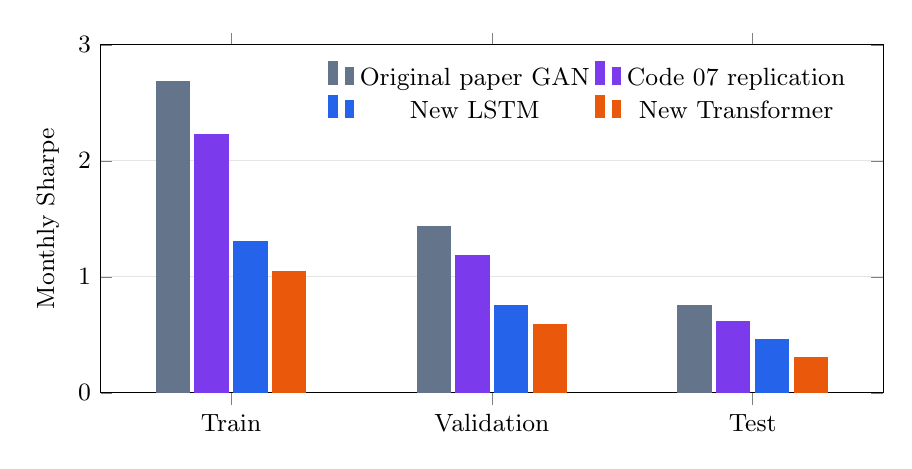
\begin{tikzpicture}
\begin{axis}[width=0.95\linewidth,height=6cm,tick label style={font=\small},label style={font=\small},legend style={font=\small,draw=none},ymajorgrids,grid style={gray!20},ybar,/pgf/bar width=12pt,ymin=0,ymax=3,xtick={0,1,2},xticklabels={Train,Validation,Test},ylabel={Monthly Sharpe},enlarge x limits=0.25,legend columns=2,legend pos=north east]
\addplot[papercolor,fill=papercolor] coordinates {(0.0000,2.680000) (1.0000,1.430000) (2.0000,0.750000)};
\addplot[repcolor,fill=repcolor] coordinates {(0.0000,2.223515) (1.0000,1.185409) (2.0000,0.611888)};
\addplot[lstmcolor,fill=lstmcolor] coordinates {(0.0000,1.307557) (1.0000,0.750136) (2.0000,0.459293)};
\addplot[transcolor,fill=transcolor] coordinates {(0.0000,1.049036) (1.0000,0.588745) (2.0000,0.304477)};\legend{Original paper GAN,Code 07 replication,New LSTM,New Transformer}\end{axis}
\end{tikzpicture}
\caption{The original paper, our historical Code 07 replication, and the new architectures. Monthly Sharpe is shown on a common scale. Both new architectures share the reduced schedule; Code 07 and the paper are historical benchmarks with different training procedures.}\label{fig:central}
\end{figure}

\begin{figure}[htbp]\centering
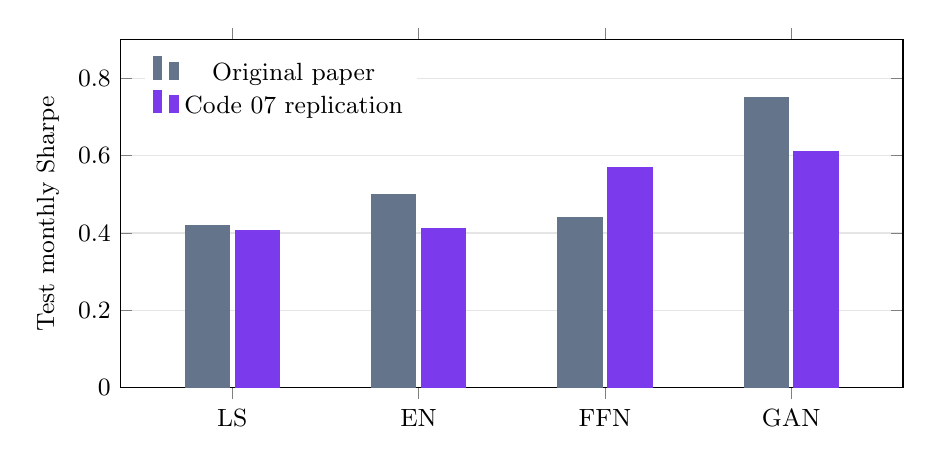
\begin{tikzpicture}
\begin{axis}[width=0.95\linewidth,height=6cm,tick label style={font=\small},label style={font=\small},legend style={font=\small,draw=none},ymajorgrids,grid style={gray!20},ybar,/pgf/bar width=16pt,ymin=0,ymax=.9,xtick={0,1,2,3},xticklabels={LS,EN,FFN,GAN},ylabel={Test monthly Sharpe},enlarge x limits=.2,legend pos=north west]
\addplot[papercolor,fill=papercolor] coordinates {(0.0000,0.420000) (1.0000,0.500000) (2.0000,0.440000) (3.0000,0.750000)};
\addplot[repcolor,fill=repcolor] coordinates {(0.0000,0.406392) (1.0000,0.411508) (2.0000,0.569521) (3.0000,0.611888)};\legend{Original paper,Code 07 replication}\end{axis}
\end{tikzpicture}
\caption{Replication check for the four original model classes, using monthly test Sharpe. Code 07 retains GAN as the strongest local model, but FFN and EN exchange positions relative to the paper.}\label{fig:replication}
\end{figure}

Figure~\ref{fig:central} makes the three layers visible. Relative to published GAN test Sharpe of 0.750, Code 07 is lower by 0.138, new LSTM by 0.291, and Transformer by 0.446. Those are contextual gaps rather than a controlled training-duration effect. The original-model check in Figure~\ref{fig:replication} is also important: LS remains close to its published benchmark, while the local FFN exceeds its benchmark and local EN is below it. Thus, preserving GAN's leading rank does not imply that every numerical result or ranking is reproduced.

\clearpage\subsection{Direct comparison with the authors' supplied factor series}
Our earlier presentation included a direct comparison with the authors' GAN factor. We use the same saved 600-month series here. Its recomputed monthly Sharpes are 2.684, 1.428, and 0.750 for training, validation, and test, close to the published rounded benchmarks. Its test correlation with the historical replication is 0.800. This permits a direct original-versus-replication comparison, beyond comparing published scalars.

\begin{table}[htbp]\centering\small\caption{Direct test-period comparison with the supplied author GAN series. Correlation is measured against that series.}\label{tab:official}\begin{tabular}{lrr}\toprule Model & Monthly Sharpe & Author correlation \\\midrule
Official GAN & 0.750 & 1.000 \\
GAN-LSTM original & 0.612 & 0.800 \\
GAN-LSTM reduced schedule & 0.459 & 0.370 \\
GAN-Transformer reduced schedule & 0.304 & 0.525 \\
50/50 blend & 0.463 & 0.565 \\
\bottomrule\end{tabular}\end{table}
The authors' mean annualized rolling Sharpes are 3.638 for 36-month windows and 3.199 for 60-month windows. Conditional monthly author Sharpes are 0.842 in expansion, 0.324 in recession, 0.598 in high volatility, and 1.003 in low volatility. These are additional diagnostics computed from the supplied author series, not statistics claimed to appear in the original paper.

\subsection{Matched LSTM versus Transformer}
Under the common reduced schedule, Transformer minus LSTM test monthly Sharpe is $-0.155$. LSTM annualized volatility is 3.87\%, compared with 4.82\% for Transformer. Mean monthly returns are approximately 0.513\% and 0.423\%, respectively. Maximum drawdowns are $-11.14\%$ and $-15.35\%$. Thus, the Transformer has both weaker average returns and greater volatility in this experiment.

The test-return correlation is approximately 0.292. A fixed 50/50 return average has test monthly Sharpe 0.463, slightly above LSTM. The small increase of about 0.004 accompanies a reduction in volatility, not an increase in mean return. Table~\ref{tab:blend} includes all sample splits. This blend was examined after reviewing test outcomes; its constant weights are not optimized on those outcomes, but the exercise is still exploratory. It is distinct from averaging raw stock weights within an architecture and introduces no extra gross-exposure renormalization.
\begin{table}[htbp]\centering\small
\caption{Monthly Sharpe for the two new architectures and an illustrative fixed 50/50 return blend.}\label{tab:blend}
\begin{tabular}{lrrr}
\toprule
Model & Train & Validation & Test \\
\midrule
LSTM & 1.308 & 0.750 & 0.459 \\
Transformer & 1.049 & 0.589 & 0.304 \\
50/50 blend & 1.414 & 0.915 & 0.463 \\
\bottomrule\end{tabular}\end{table}


\begin{figure}[htbp]\centering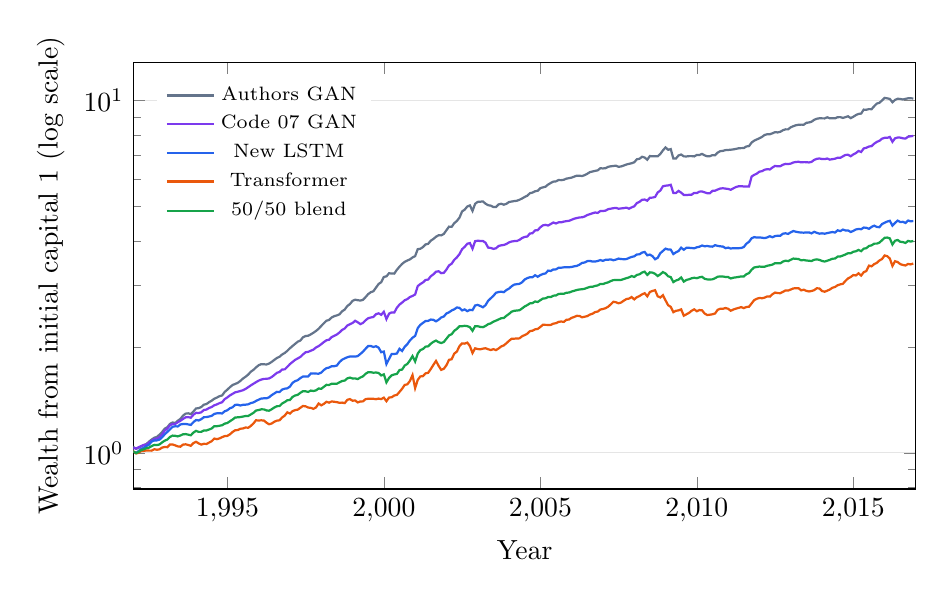
\begin{tikzpicture}
\begin{axis}[width=.95\linewidth,height=7cm,xmin=1992,xmax=2017,xtick={1995,2000,2005,2010,2015},ymode=log,ymajorgrids,grid style={gray!20},ylabel={Wealth from initial capital 1 (log scale)},xlabel={Year},legend style={font=\scriptsize,draw=none},legend pos=north west]
\addplot[papercolor,thick,no marks] coordinates {(1991.9167,1.000000) (1992.0000,1.038359) (1992.0833,1.026499) (1992.1667,1.033478) (1992.2500,1.043647) (1992.3333,1.052090) (1992.4167,1.059609) (1992.5000,1.076620) (1992.5833,1.091503) (1992.6667,1.104077) (1992.7500,1.110136) (1992.8333,1.126427) (1992.9167,1.146575) (1993.0000,1.171248) (1993.0833,1.183001) (1993.1667,1.208340) (1993.2500,1.219928) (1993.3333,1.215167) (1993.4167,1.233757) (1993.5000,1.248466) (1993.5833,1.275352) (1993.6667,1.292186) (1993.7500,1.295128) (1993.8333,1.288098) (1993.9167,1.310634) (1994.0000,1.336731) (1994.0833,1.339783) (1994.1667,1.349565) (1994.2500,1.370376) (1994.3333,1.375875) (1994.4167,1.393096) (1994.5000,1.406769) (1994.5833,1.424755) (1994.6667,1.435481) (1994.7500,1.448885) (1994.8333,1.455818) (1994.9167,1.489678) (1995.0000,1.511902) (1995.0833,1.536462) (1995.1667,1.558275) (1995.2500,1.569293) (1995.3333,1.580865) (1995.4167,1.600830) (1995.5000,1.625842) (1995.5833,1.645325) (1995.6667,1.668417) (1995.7500,1.700131) (1995.8333,1.720626) (1995.9167,1.748480) (1996.0000,1.773433) (1996.0833,1.786477) (1996.1667,1.784541) (1996.2500,1.782722) (1996.3333,1.792606) (1996.4167,1.812718) (1996.5000,1.836478) (1996.5833,1.859447) (1996.6667,1.874705) (1996.7500,1.902586) (1996.8333,1.921700) (1996.9167,1.948781) (1997.0000,1.981902) (1997.0833,2.010911) (1997.1667,2.040027) (1997.2500,2.068532) (1997.3333,2.084296) (1997.4167,2.129283) (1997.5000,2.146358) (1997.5833,2.151638) (1997.6667,2.170256) (1997.7500,2.193364) (1997.8333,2.219098) (1997.9167,2.251024) (1998.0000,2.292584) (1998.0833,2.334146) (1998.1667,2.372279) (1998.2500,2.385038) (1998.3333,2.423740) (1998.4167,2.444956) (1998.5000,2.456630) (1998.5833,2.473512) (1998.6667,2.523424) (1998.7500,2.552197) (1998.8333,2.612066) (1998.9167,2.645766) (1999.0000,2.701992) (1999.0833,2.722569) (1999.1667,2.713755) (1999.2500,2.706506) (1999.3333,2.720226) (1999.4167,2.768606) (1999.5000,2.823872) (1999.5833,2.859085) (1999.6667,2.876823) (1999.7500,2.946885) (1999.8333,3.016615) (1999.9167,3.051134) (2000.0000,3.158107) (2000.0833,3.171636) (2000.1667,3.236385) (2000.2500,3.230931) (2000.3333,3.228496) (2000.4167,3.310987) (2000.5000,3.377721) (2000.5833,3.439513) (2000.6667,3.487727) (2000.7500,3.517911) (2000.8333,3.542892) (2000.9167,3.589425) (2001.0000,3.620065) (2001.0833,3.788784) (2001.1667,3.798756) (2001.2500,3.841726) (2001.3333,3.907876) (2001.4167,3.923819) (2001.5000,4.003996) (2001.5833,4.049328) (2001.6667,4.109124) (2001.7500,4.148003) (2001.8333,4.145403) (2001.9167,4.185959) (2002.0000,4.287680) (2002.0833,4.389803) (2002.1667,4.382691) (2002.2500,4.490791) (2002.3333,4.554237) (2002.4167,4.654876) (2002.5000,4.847399) (2002.5833,4.905110) (2002.6667,5.006823) (2002.7500,5.042953) (2002.8333,4.864216) (2002.9167,5.095843) (2003.0000,5.161115) (2003.0833,5.167628) (2003.1667,5.175385) (2003.2500,5.099120) (2003.3333,5.049847) (2003.4167,5.035428) (2003.5000,4.991223) (2003.5833,4.990843) (2003.6667,5.076553) (2003.7500,5.098552) (2003.8333,5.066684) (2003.9167,5.096075) (2004.0000,5.155568) (2004.0833,5.171997) (2004.1667,5.188201) (2004.2500,5.198450) (2004.3333,5.232665) (2004.4167,5.276786) (2004.5000,5.328626) (2004.5833,5.371928) (2004.6667,5.462038) (2004.7500,5.483515) (2004.8333,5.531646) (2004.9167,5.551137) (2005.0000,5.645428) (2005.0833,5.674612) (2005.1667,5.700280) (2005.2500,5.781289) (2005.3333,5.839876) (2005.4167,5.890817) (2005.5000,5.901444) (2005.5833,5.951982) (2005.6667,5.948708) (2005.7500,5.963928) (2005.8333,6.007887) (2005.9167,6.027042) (2006.0000,6.047967) (2006.0833,6.088675) (2006.1667,6.124694) (2006.2500,6.122930) (2006.3333,6.112561) (2006.4167,6.147267) (2006.5000,6.201489) (2006.5833,6.269872) (2006.6667,6.295010) (2006.7500,6.320818) (2006.8333,6.342367) (2006.9167,6.430054) (2007.0000,6.422988) (2007.0833,6.434142) (2007.1667,6.489875) (2007.2500,6.512075) (2007.3333,6.525978) (2007.4167,6.539778) (2007.5000,6.488964) (2007.5833,6.508720) (2007.6667,6.546670) (2007.7500,6.589288) (2007.8333,6.617498) (2007.9167,6.645323) (2008.0000,6.684328) (2008.0833,6.818969) (2008.1667,6.841255) (2008.2500,6.931557) (2008.3333,6.897540) (2008.4167,6.800056) (2008.5000,6.965355) (2008.5833,6.951786) (2008.6667,6.957685) (2008.7500,6.953875) (2008.8333,7.057650) (2008.9167,7.227563) (2009.0000,7.368711) (2009.0833,7.255282) (2009.1667,7.288816) (2009.2500,6.851385) (2009.3333,6.851758) (2009.4167,6.993153) (2009.5000,7.034663) (2009.5833,6.950892) (2009.6667,6.946357) (2009.7500,6.960107) (2009.8333,6.961086) (2009.9167,6.948868) (2010.0000,7.016194) (2010.0833,7.012940) (2010.1667,7.062094) (2010.2500,6.995778) (2010.3333,6.953241) (2010.4167,6.956874) (2010.5000,7.006639) (2010.5833,7.003823) (2010.6667,7.124774) (2010.7500,7.191787) (2010.8333,7.206365) (2010.9167,7.240373) (2011.0000,7.247792) (2011.0833,7.258659) (2011.1667,7.274569) (2011.2500,7.298654) (2011.3333,7.325911) (2011.4167,7.335134) (2011.5000,7.336371) (2011.5833,7.415490) (2011.6667,7.432738) (2011.7500,7.608169) (2011.8333,7.703431) (2011.9167,7.763736) (2012.0000,7.822575) (2012.0833,7.895630) (2012.1667,7.995217) (2012.2500,8.031140) (2012.3333,8.032284) (2012.4167,8.080982) (2012.5000,8.142413) (2012.5833,8.126556) (2012.6667,8.161699) (2012.7500,8.242926) (2012.8333,8.292015) (2012.9167,8.291897) (2013.0000,8.404358) (2013.0833,8.465986) (2013.1667,8.518904) (2013.2500,8.545417) (2013.3333,8.552131) (2013.4167,8.548186) (2013.5000,8.653847) (2013.5833,8.672892) (2013.6667,8.717241) (2013.7500,8.826186) (2013.8333,8.889372) (2013.9167,8.914847) (2014.0000,8.910690) (2014.0833,8.907858) (2014.1667,8.973229) (2014.2500,8.911587) (2014.3333,8.922599) (2014.4167,8.910821) (2014.5000,8.980390) (2014.5833,8.982646) (2014.6667,8.936058) (2014.7500,8.979866) (2014.8333,9.031274) (2014.9167,8.921701) (2015.0000,9.005180) (2015.0833,9.102496) (2015.1667,9.174022) (2015.2500,9.194898) (2015.3333,9.435111) (2015.4167,9.427734) (2015.5000,9.466268) (2015.5833,9.461778) (2015.6667,9.645523) (2015.7500,9.811012) (2015.8333,9.864812) (2015.9167,10.015697) (2016.0000,10.183787) (2016.0833,10.156221) (2016.1667,10.117683) (2016.2500,9.899492) (2016.3333,10.056055) (2016.4167,10.127817) (2016.5000,10.117404) (2016.5833,10.080262) (2016.6667,10.120119) (2016.7500,10.158926) (2016.8333,10.159545) (2016.9167,10.148117)};
\addplot[repcolor,thick,no marks] coordinates {(1991.9167,1.000000) (1992.0000,1.033364) (1992.0833,1.028745) (1992.1667,1.037615) (1992.2500,1.045500) (1992.3333,1.053259) (1992.4167,1.055753) (1992.5000,1.070356) (1992.5833,1.082653) (1992.6667,1.094034) (1992.7500,1.098332) (1992.8333,1.107486) (1992.9167,1.127936) (1993.0000,1.157157) (1993.0833,1.172387) (1993.1667,1.196563) (1993.2500,1.208448) (1993.3333,1.207999) (1993.4167,1.221426) (1993.5000,1.233069) (1993.5833,1.248229) (1993.6667,1.261478) (1993.7500,1.263515) (1993.8333,1.258484) (1993.9167,1.283354) (1994.0000,1.299386) (1994.0833,1.297587) (1994.1667,1.303838) (1994.2500,1.323239) (1994.3333,1.327321) (1994.4167,1.340936) (1994.5000,1.349627) (1994.5833,1.364890) (1994.6667,1.372830) (1994.7500,1.384353) (1994.8333,1.392621) (1994.9167,1.421371) (1995.0000,1.437112) (1995.0833,1.456198) (1995.1667,1.470689) (1995.2500,1.485528) (1995.3333,1.491580) (1995.4167,1.498545) (1995.5000,1.506437) (1995.5833,1.518985) (1995.6667,1.536511) (1995.7500,1.554887) (1995.8333,1.571320) (1995.9167,1.587966) (1996.0000,1.603552) (1996.0833,1.614952) (1996.1667,1.622056) (1996.2500,1.622706) (1996.3333,1.627085) (1996.4167,1.642016) (1996.5000,1.663420) (1996.5833,1.687940) (1996.6667,1.697182) (1996.7500,1.724830) (1996.8333,1.726503) (1996.9167,1.754977) (1997.0000,1.786857) (1997.0833,1.812047) (1997.1667,1.837168) (1997.2500,1.854470) (1997.3333,1.872483) (1997.4167,1.903187) (1997.5000,1.930668) (1997.5833,1.936084) (1997.6667,1.950593) (1997.7500,1.964686) (1997.8333,1.992102) (1997.9167,2.009353) (1998.0000,2.035285) (1998.0833,2.063619) (1998.1667,2.087987) (1998.2500,2.095436) (1998.3333,2.131667) (1998.4167,2.149424) (1998.5000,2.168033) (1998.5833,2.197769) (1998.6667,2.233575) (1998.7500,2.255120) (1998.8333,2.299800) (1998.9167,2.319225) (1999.0000,2.337259) (1999.0833,2.371533) (1999.1667,2.349180) (1999.2500,2.320188) (1999.3333,2.338820) (1999.4167,2.379513) (1999.5000,2.411487) (1999.5833,2.423037) (1999.6667,2.431553) (1999.7500,2.476785) (1999.8333,2.490283) (1999.9167,2.466508) (2000.0000,2.515402) (2000.0833,2.397837) (2000.1667,2.484087) (2000.2500,2.505426) (2000.3333,2.502909) (2000.4167,2.582399) (2000.5000,2.636802) (2000.5833,2.670928) (2000.6667,2.712417) (2000.7500,2.732653) (2000.8333,2.770258) (2000.9167,2.790552) (2001.0000,2.816533) (2001.0833,2.974487) (2001.1667,3.016795) (2001.2500,3.046945) (2001.3333,3.096746) (2001.4167,3.105794) (2001.5000,3.173408) (2001.5833,3.214215) (2001.6667,3.268740) (2001.7500,3.279402) (2001.8333,3.238284) (2001.9167,3.244695) (2002.0000,3.315538) (2002.0833,3.406002) (2002.1667,3.445351) (2002.2500,3.533407) (2002.3333,3.590095) (2002.4167,3.668873) (2002.5000,3.787292) (2002.5833,3.846858) (2002.6667,3.924776) (2002.7500,3.943246) (2002.8333,3.799980) (2002.9167,3.991126) (2003.0000,4.004144) (2003.0833,3.997151) (2003.1667,3.997333) (2003.2500,3.950629) (2003.3333,3.826877) (2003.4167,3.819446) (2003.5000,3.795705) (2003.5833,3.809893) (2003.6667,3.868125) (2003.7500,3.885048) (2003.8333,3.893746) (2003.9167,3.919583) (2004.0000,3.961173) (2004.0833,3.983311) (2004.1667,3.994236) (2004.2500,3.996553) (2004.3333,4.025254) (2004.4167,4.074580) (2004.5000,4.103883) (2004.5833,4.114431) (2004.6667,4.196703) (2004.7500,4.205261) (2004.8333,4.283611) (2004.9167,4.289043) (2005.0000,4.371658) (2005.0833,4.426406) (2005.1667,4.441386) (2005.2500,4.420783) (2005.3333,4.465384) (2005.4167,4.509578) (2005.5000,4.481747) (2005.5833,4.514340) (2005.6667,4.514149) (2005.7500,4.536695) (2005.8333,4.550521) (2005.9167,4.559953) (2006.0000,4.591256) (2006.0833,4.623741) (2006.1667,4.642865) (2006.2500,4.661784) (2006.3333,4.665303) (2006.4167,4.691159) (2006.5000,4.734690) (2006.5833,4.762365) (2006.6667,4.790969) (2006.7500,4.814467) (2006.8333,4.802723) (2006.9167,4.858765) (2007.0000,4.861167) (2007.0833,4.873511) (2007.1667,4.920081) (2007.2500,4.936412) (2007.3333,4.952332) (2007.4167,4.961263) (2007.5000,4.934310) (2007.5833,4.944860) (2007.6667,4.954535) (2007.7500,4.969475) (2007.8333,4.935910) (2007.9167,4.977974) (2008.0000,5.012296) (2008.0833,5.120945) (2008.1667,5.159970) (2008.2500,5.231768) (2008.3333,5.240108) (2008.4167,5.201561) (2008.5000,5.302439) (2008.5833,5.306706) (2008.6667,5.330042) (2008.7500,5.489445) (2008.8333,5.556053) (2008.9167,5.714127) (2009.0000,5.736602) (2009.0833,5.746293) (2009.1667,5.771929) (2009.2500,5.472684) (2009.3333,5.468791) (2009.4167,5.545558) (2009.5000,5.482857) (2009.5833,5.400718) (2009.6667,5.396307) (2009.7500,5.405686) (2009.8333,5.409456) (2009.9167,5.473060) (2010.0000,5.467004) (2010.0833,5.518794) (2010.1667,5.523342) (2010.2500,5.491544) (2010.3333,5.460581) (2010.4167,5.460678) (2010.5000,5.547203) (2010.5833,5.553129) (2010.6667,5.595362) (2010.7500,5.631711) (2010.8333,5.641138) (2010.9167,5.628723) (2011.0000,5.615781) (2011.0833,5.585153) (2011.1667,5.639030) (2011.2500,5.687383) (2011.3333,5.714272) (2011.4167,5.720993) (2011.5000,5.706781) (2011.5833,5.709472) (2011.6667,5.705932) (2011.7500,6.089371) (2011.8333,6.158045) (2011.9167,6.208038) (2012.0000,6.288539) (2012.0833,6.309367) (2012.1667,6.368828) (2012.2500,6.390870) (2012.3333,6.379058) (2012.4167,6.461762) (2012.5000,6.530042) (2012.5833,6.511871) (2012.6667,6.515773) (2012.7500,6.581001) (2012.8333,6.617800) (2012.9167,6.608359) (2013.0000,6.627827) (2013.0833,6.677176) (2013.1667,6.699337) (2013.2500,6.709831) (2013.3333,6.682688) (2013.4167,6.693462) (2013.5000,6.690779) (2013.5833,6.678281) (2013.6667,6.704879) (2013.7500,6.790862) (2013.8333,6.838056) (2013.9167,6.854901) (2014.0000,6.829102) (2014.0833,6.825899) (2014.1667,6.852898) (2014.2500,6.802298) (2014.3333,6.825714) (2014.4167,6.844995) (2014.5000,6.888865) (2014.5833,6.883436) (2014.6667,6.950203) (2014.7500,7.016377) (2014.8333,7.021950) (2014.9167,6.956709) (2015.0000,7.039804) (2015.0833,7.102447) (2015.1667,7.198072) (2015.2500,7.153085) (2015.3333,7.321744) (2015.4167,7.350767) (2015.5000,7.412580) (2015.5833,7.431262) (2015.6667,7.551767) (2015.7500,7.640106) (2015.8333,7.694066) (2015.9167,7.803744) (2016.0000,7.845575) (2016.0833,7.844222) (2016.1667,7.891628) (2016.2500,7.646185) (2016.3333,7.821349) (2016.4167,7.860350) (2016.5000,7.856999) (2016.5833,7.822307) (2016.6667,7.807374) (2016.7500,7.903299) (2016.8333,7.926389) (2016.9167,7.943595)};
\addplot[lstmcolor,thick,no marks] coordinates {(1991.9167,1.000000) (1992.0000,1.007048) (1992.0833,1.000567) (1992.1667,1.011974) (1992.2500,1.025849) (1992.3333,1.033989) (1992.4167,1.046203) (1992.5000,1.055419) (1992.5833,1.077150) (1992.6667,1.084093) (1992.7500,1.084992) (1992.8333,1.090475) (1992.9167,1.107281) (1993.0000,1.128845) (1993.0833,1.146906) (1993.1667,1.165624) (1993.2500,1.186161) (1993.3333,1.189707) (1993.4167,1.188468) (1993.5000,1.204030) (1993.5833,1.207418) (1993.6667,1.208038) (1993.7500,1.204417) (1993.8333,1.200501) (1993.9167,1.222518) (1994.0000,1.239510) (1994.0833,1.235969) (1994.1667,1.245974) (1994.2500,1.262850) (1994.3333,1.263444) (1994.4167,1.268223) (1994.5000,1.273735) (1994.5833,1.290097) (1994.6667,1.295055) (1994.7500,1.296030) (1994.8333,1.293989) (1994.9167,1.312693) (1995.0000,1.321328) (1995.0833,1.338806) (1995.1667,1.347308) (1995.2500,1.368522) (1995.3333,1.369875) (1995.4167,1.362983) (1995.5000,1.369057) (1995.5833,1.370444) (1995.6667,1.373593) (1995.7500,1.384568) (1995.8333,1.390739) (1995.9167,1.404189) (1996.0000,1.415807) (1996.0833,1.426568) (1996.1667,1.428406) (1996.2500,1.428220) (1996.3333,1.438172) (1996.4167,1.458645) (1996.5000,1.474539) (1996.5833,1.490390) (1996.6667,1.488469) (1996.7500,1.512130) (1996.8333,1.521300) (1996.9167,1.524719) (1997.0000,1.542424) (1997.0833,1.580715) (1997.1667,1.598891) (1997.2500,1.608700) (1997.3333,1.631265) (1997.4167,1.646960) (1997.5000,1.647436) (1997.5833,1.648193) (1997.6667,1.680364) (1997.7500,1.681676) (1997.8333,1.679545) (1997.9167,1.678084) (1998.0000,1.690151) (1998.0833,1.718766) (1998.1667,1.740238) (1998.2500,1.746884) (1998.3333,1.761975) (1998.4167,1.762777) (1998.5000,1.770188) (1998.5833,1.810364) (1998.6667,1.839042) (1998.7500,1.854687) (1998.8333,1.868787) (1998.9167,1.878097) (1999.0000,1.878136) (1999.0833,1.876617) (1999.1667,1.883001) (1999.2500,1.909423) (1999.3333,1.938343) (1999.4167,1.975754) (1999.5000,2.011114) (1999.5833,2.011234) (1999.6667,1.998391) (1999.7500,2.008489) (1999.8333,1.989450) (1999.9167,1.930963) (2000.0000,1.940342) (2000.0833,1.787225) (2000.1667,1.848122) (2000.2500,1.909300) (2000.3333,1.908992) (2000.4167,1.914818) (2000.5000,1.975094) (2000.5833,1.947044) (2000.6667,2.000976) (2000.7500,2.035359) (2000.8333,2.084879) (2000.9167,2.122669) (2001.0000,2.148507) (2001.0833,2.259802) (2001.1667,2.309942) (2001.2500,2.339239) (2001.3333,2.368196) (2001.4167,2.370586) (2001.5000,2.390888) (2001.5833,2.386356) (2001.6667,2.362817) (2001.7500,2.387858) (2001.8333,2.423534) (2001.9167,2.438806) (2002.0000,2.487616) (2002.0833,2.507156) (2002.1667,2.537006) (2002.2500,2.556400) (2002.3333,2.587482) (2002.4167,2.580921) (2002.5000,2.537712) (2002.5833,2.555381) (2002.6667,2.526291) (2002.7500,2.547457) (2002.8333,2.542377) (2002.9167,2.621164) (2003.0000,2.631436) (2003.0833,2.611980) (2003.1667,2.590996) (2003.2500,2.627541) (2003.3333,2.703610) (2003.4167,2.747435) (2003.5000,2.791698) (2003.5833,2.848285) (2003.6667,2.862186) (2003.7500,2.869019) (2003.8333,2.859518) (2003.9167,2.900253) (2004.0000,2.926978) (2004.0833,2.972707) (2004.1667,3.004954) (2004.2500,3.013021) (2004.3333,3.020350) (2004.4167,3.050797) (2004.5000,3.106562) (2004.5833,3.135188) (2004.6667,3.152480) (2004.7500,3.153289) (2004.8333,3.194616) (2004.9167,3.162914) (2005.0000,3.197431) (2005.0833,3.220219) (2005.1667,3.233084) (2005.2500,3.292739) (2005.3333,3.284895) (2005.4167,3.318555) (2005.5000,3.319208) (2005.5833,3.354431) (2005.6667,3.356258) (2005.7500,3.364036) (2005.8333,3.363641) (2005.9167,3.365673) (2006.0000,3.373109) (2006.0833,3.386119) (2006.1667,3.396475) (2006.2500,3.422347) (2006.3333,3.463094) (2006.4167,3.471997) (2006.5000,3.503333) (2006.5833,3.508747) (2006.6667,3.493970) (2006.7500,3.494136) (2006.8333,3.506100) (2006.9167,3.528054) (2007.0000,3.509449) (2007.0833,3.534844) (2007.1667,3.536253) (2007.2500,3.542735) (2007.3333,3.523347) (2007.4167,3.538634) (2007.5000,3.562251) (2007.5833,3.550806) (2007.6667,3.547781) (2007.7500,3.549798) (2007.8333,3.577618) (2007.9167,3.601237) (2008.0000,3.614947) (2008.0833,3.659548) (2008.1667,3.662917) (2008.2500,3.705341) (2008.3333,3.720723) (2008.4167,3.639103) (2008.5000,3.657175) (2008.5833,3.618457) (2008.6667,3.547119) (2008.7500,3.580441) (2008.8333,3.690985) (2008.9167,3.744706) (2009.0000,3.802375) (2009.0833,3.781178) (2009.1667,3.777636) (2009.2500,3.669247) (2009.3333,3.711102) (2009.4167,3.743926) (2009.5000,3.825718) (2009.5833,3.774574) (2009.6667,3.822821) (2009.7500,3.822117) (2009.8333,3.817134) (2009.9167,3.808489) (2010.0000,3.834805) (2010.0833,3.849682) (2010.1667,3.880278) (2010.2500,3.860935) (2010.3333,3.868878) (2010.4167,3.855996) (2010.5000,3.851555) (2010.5833,3.888916) (2010.6667,3.870425) (2010.7500,3.859942) (2010.8333,3.853964) (2010.9167,3.814106) (2011.0000,3.827393) (2011.0833,3.804154) (2011.1667,3.814552) (2011.2500,3.809035) (2011.3333,3.812211) (2011.4167,3.817772) (2011.5000,3.841202) (2011.5833,3.926434) (2011.6667,3.974448) (2011.7500,4.067842) (2011.8333,4.099185) (2011.9167,4.086161) (2012.0000,4.091517) (2012.0833,4.082799) (2012.1667,4.072262) (2012.2500,4.090825) (2012.3333,4.123365) (2012.4167,4.094934) (2012.5000,4.126576) (2012.5833,4.136682) (2012.6667,4.135745) (2012.7500,4.190679) (2012.8333,4.203019) (2012.9167,4.184910) (2013.0000,4.229909) (2013.0833,4.265902) (2013.1667,4.245462) (2013.2500,4.230708) (2013.3333,4.222645) (2013.4167,4.219999) (2013.5000,4.225157) (2013.5833,4.227662) (2013.6667,4.200844) (2013.7500,4.244147) (2013.8333,4.214824) (2013.9167,4.192166) (2014.0000,4.202081) (2014.0833,4.191441) (2014.1667,4.207429) (2014.2500,4.223721) (2014.3333,4.236508) (2014.4167,4.223655) (2014.5000,4.285087) (2014.5833,4.263936) (2014.6667,4.304851) (2014.7500,4.280916) (2014.8333,4.282534) (2014.9167,4.238439) (2015.0000,4.269394) (2015.0833,4.309387) (2015.1667,4.323025) (2015.2500,4.316009) (2015.3333,4.362985) (2015.4167,4.356531) (2015.5000,4.327077) (2015.5833,4.381707) (2015.6667,4.417184) (2015.7500,4.381895) (2015.8333,4.372389) (2015.9167,4.464361) (2016.0000,4.503690) (2016.0833,4.538105) (2016.1667,4.560523) (2016.2500,4.417311) (2016.3333,4.498280) (2016.4167,4.565956) (2016.5000,4.523503) (2016.5833,4.529946) (2016.6667,4.496268) (2016.7500,4.568769) (2016.8333,4.544627) (2016.9167,4.552737)};
\addplot[transcolor,thick,no marks] coordinates {(1991.9167,1.000000) (1992.0000,1.009809) (1992.0833,0.996059) (1992.1667,1.000771) (1992.2500,1.011714) (1992.3333,1.012991) (1992.4167,1.016142) (1992.5000,1.014661) (1992.5833,1.014599) (1992.6667,1.024033) (1992.7500,1.020534) (1992.8333,1.023573) (1992.9167,1.035254) (1993.0000,1.039220) (1993.0833,1.037911) (1993.1667,1.056380) (1993.2500,1.056183) (1993.3333,1.050242) (1993.4167,1.043362) (1993.5000,1.041212) (1993.5833,1.055555) (1993.6667,1.057565) (1993.7500,1.053103) (1993.8333,1.047357) (1993.9167,1.066202) (1994.0000,1.075023) (1994.0833,1.063932) (1994.1667,1.055639) (1994.2500,1.060858) (1994.3333,1.060209) (1994.4167,1.069436) (1994.5000,1.079313) (1994.5833,1.098126) (1994.6667,1.093612) (1994.7500,1.099255) (1994.8333,1.108307) (1994.9167,1.115807) (1995.0000,1.117354) (1995.0833,1.128931) (1995.1667,1.146308) (1995.2500,1.159078) (1995.3333,1.161175) (1995.4167,1.170675) (1995.5000,1.173048) (1995.5833,1.180273) (1995.6667,1.178524) (1995.7500,1.192400) (1995.8333,1.211977) (1995.9167,1.237460) (1996.0000,1.235522) (1996.0833,1.237214) (1996.1667,1.235338) (1996.2500,1.218538) (1996.3333,1.205395) (1996.4167,1.211331) (1996.5000,1.225742) (1996.5833,1.234242) (1996.6667,1.237291) (1996.7500,1.259824) (1996.8333,1.275876) (1996.9167,1.303338) (1997.0000,1.293153) (1997.0833,1.313366) (1997.1667,1.322422) (1997.2500,1.326571) (1997.3333,1.342843) (1997.4167,1.358718) (1997.5000,1.355809) (1997.5833,1.344726) (1997.6667,1.341935) (1997.7500,1.333625) (1997.8333,1.345909) (1997.9167,1.380496) (1998.0000,1.364580) (1998.0833,1.377362) (1998.1667,1.396430) (1998.2500,1.388702) (1998.3333,1.399764) (1998.4167,1.396472) (1998.5000,1.393235) (1998.5833,1.386968) (1998.6667,1.389157) (1998.7500,1.384479) (1998.8333,1.414394) (1998.9167,1.421501) (1999.0000,1.406169) (1999.0833,1.408726) (1999.1667,1.390437) (1999.2500,1.399644) (1999.3333,1.400270) (1999.4167,1.420866) (1999.5000,1.424465) (1999.5833,1.424379) (1999.6667,1.423936) (1999.7500,1.420576) (1999.8333,1.425915) (1999.9167,1.421687) (2000.0000,1.434768) (2000.0833,1.402016) (2000.1667,1.435633) (2000.2500,1.438659) (2000.3333,1.454996) (2000.4167,1.460751) (2000.5000,1.489607) (2000.5833,1.520524) (2000.6667,1.559286) (2000.7500,1.565164) (2000.8333,1.599686) (2000.9167,1.663168) (2001.0000,1.527591) (2001.0833,1.611140) (2001.1667,1.648359) (2001.2500,1.651467) (2001.3333,1.682266) (2001.4167,1.687898) (2001.5000,1.730428) (2001.5833,1.777745) (2001.6667,1.824353) (2001.7500,1.767190) (2001.8333,1.720626) (2001.9167,1.733094) (2002.0000,1.773442) (2002.0833,1.837255) (2002.1667,1.844696) (2002.2500,1.913868) (2002.3333,1.939256) (2002.4167,2.009571) (2002.5000,2.045676) (2002.5833,2.042526) (2002.6667,2.056431) (2002.7500,2.010916) (2002.8333,1.921379) (2002.9167,1.981022) (2003.0000,1.971757) (2003.0833,1.967967) (2003.1667,1.977128) (2003.2500,1.981953) (2003.3333,1.969314) (2003.4167,1.959532) (2003.5000,1.970517) (2003.5833,1.958303) (2003.6667,1.979100) (2003.7500,2.005244) (2003.8333,2.018925) (2003.9167,2.048168) (2004.0000,2.080266) (2004.0833,2.109005) (2004.1667,2.110175) (2004.2500,2.111981) (2004.3333,2.114434) (2004.4167,2.143248) (2004.5000,2.160202) (2004.5833,2.179019) (2004.6667,2.215939) (2004.7500,2.223098) (2004.8333,2.242980) (2004.9167,2.248689) (2005.0000,2.278034) (2005.0833,2.310470) (2005.1667,2.309324) (2005.2500,2.308235) (2005.3333,2.308887) (2005.4167,2.327388) (2005.5000,2.335026) (2005.5833,2.354731) (2005.6667,2.360755) (2005.7500,2.354112) (2005.8333,2.387025) (2005.9167,2.390985) (2006.0000,2.418137) (2006.0833,2.432256) (2006.1667,2.449880) (2006.2500,2.448061) (2006.3333,2.426013) (2006.4167,2.435498) (2006.5000,2.445135) (2006.5833,2.469734) (2006.6667,2.483305) (2006.7500,2.510626) (2006.8333,2.519138) (2006.9167,2.552681) (2007.0000,2.561716) (2007.0833,2.575409) (2007.1667,2.599908) (2007.2500,2.640165) (2007.3333,2.686487) (2007.4167,2.677243) (2007.5000,2.658941) (2007.5833,2.673327) (2007.6667,2.705373) (2007.7500,2.733813) (2007.8333,2.741757) (2007.9167,2.769986) (2008.0000,2.727967) (2008.0833,2.766793) (2008.1667,2.787051) (2008.2500,2.819092) (2008.3333,2.840381) (2008.4167,2.783075) (2008.5000,2.863621) (2008.5833,2.882829) (2008.6667,2.896362) (2008.7500,2.784221) (2008.8333,2.762251) (2008.9167,2.803344) (2009.0000,2.710660) (2009.0833,2.625971) (2009.1667,2.598245) (2009.2500,2.508662) (2009.3333,2.531210) (2009.4167,2.538632) (2009.5000,2.555536) (2009.5833,2.451729) (2009.6667,2.474303) (2009.7500,2.496766) (2009.8333,2.532475) (2009.9167,2.555992) (2010.0000,2.524290) (2010.0833,2.543801) (2010.1667,2.539673) (2010.2500,2.486859) (2010.3333,2.462431) (2010.4167,2.467994) (2010.5000,2.474965) (2010.5833,2.487689) (2010.6667,2.548368) (2010.7500,2.565620) (2010.8333,2.565416) (2010.9167,2.577795) (2011.0000,2.565558) (2011.0833,2.532621) (2011.1667,2.552538) (2011.2500,2.567912) (2011.3333,2.580182) (2011.4167,2.593483) (2011.5000,2.576492) (2011.5833,2.595265) (2011.6667,2.600315) (2011.7500,2.656210) (2011.8333,2.715439) (2011.9167,2.738766) (2012.0000,2.753480) (2012.0833,2.748276) (2012.1667,2.759488) (2012.2500,2.781709) (2012.3333,2.777845) (2012.4167,2.821666) (2012.5000,2.852097) (2012.5833,2.842749) (2012.6667,2.840758) (2012.7500,2.865428) (2012.8333,2.892108) (2012.9167,2.888884) (2013.0000,2.909426) (2013.0833,2.930354) (2013.1667,2.936056) (2013.2500,2.935802) (2013.3333,2.894158) (2013.4167,2.906154) (2013.5000,2.884051) (2013.5833,2.873343) (2013.6667,2.882007) (2013.7500,2.898074) (2013.8333,2.933582) (2013.9167,2.929674) (2014.0000,2.881528) (2014.0833,2.868061) (2014.1667,2.887858) (2014.2500,2.910238) (2014.3333,2.943506) (2014.4167,2.958806) (2014.5000,2.992969) (2014.5833,3.009737) (2014.6667,3.020600) (2014.7500,3.079513) (2014.8333,3.129422) (2014.9167,3.157989) (2015.0000,3.198319) (2015.0833,3.189632) (2015.1667,3.234678) (2015.2500,3.187978) (2015.3333,3.259527) (2015.4167,3.283872) (2015.5000,3.402363) (2015.5833,3.386155) (2015.6667,3.435572) (2015.7500,3.463238) (2015.8333,3.518177) (2015.9167,3.550973) (2016.0000,3.635572) (2016.0833,3.618526) (2016.1667,3.562673) (2016.2500,3.395136) (2016.3333,3.501060) (2016.4167,3.482812) (2016.5000,3.435449) (2016.5833,3.416636) (2016.6667,3.404586) (2016.7500,3.439895) (2016.8333,3.429043) (2016.9167,3.449759)};
\addplot[blendcolor,thick,no marks] coordinates {(1991.9167,1.000000) (1992.0000,1.008429) (1992.0833,0.998318) (1992.1667,1.006370) (1992.2500,1.018771) (1992.3333,1.023456) (1992.4167,1.031093) (1992.5000,1.034883) (1992.5833,1.045505) (1992.6667,1.053735) (1992.7500,1.052372) (1992.8333,1.056598) (1992.9167,1.070769) (1993.0000,1.083246) (1993.0833,1.091230) (1993.1667,1.109843) (1993.2500,1.119517) (1993.3333,1.118042) (1993.4167,1.113797) (1993.5000,1.119942) (1993.5833,1.129231) (1993.6667,1.130597) (1993.7500,1.126517) (1993.8333,1.121612) (1993.9167,1.141988) (1994.0000,1.154649) (1994.0833,1.147043) (1994.1667,1.147215) (1994.2500,1.157820) (1994.3333,1.157738) (1994.4167,1.164966) (1994.5000,1.172877) (1994.5833,1.190632) (1994.6667,1.190473) (1994.7500,1.193992) (1994.8333,1.197969) (1994.9167,1.210680) (1995.0000,1.215501) (1995.0833,1.229837) (1995.1667,1.243207) (1995.2500,1.259920) (1995.3333,1.261682) (1995.4167,1.263669) (1995.5000,1.267766) (1995.5833,1.272312) (1995.6667,1.272831) (1995.7500,1.285409) (1995.8333,1.298826) (1995.9167,1.318761) (1996.0000,1.323184) (1996.0833,1.329119) (1996.1667,1.328967) (1996.2500,1.319844) (1996.3333,1.317325) (1996.4167,1.329944) (1996.5000,1.345101) (1996.5833,1.356995) (1996.6667,1.357796) (1996.7500,1.380952) (1996.8333,1.393937) (1996.9167,1.410505) (1997.0000,1.413183) (1997.0833,1.441769) (1997.1667,1.455029) (1997.2500,1.461775) (1997.3333,1.480992) (1997.4167,1.496870) (1997.5000,1.495485) (1997.5833,1.489716) (1997.6667,1.502708) (1997.7500,1.498642) (1997.8333,1.504595) (1997.9167,1.523273) (1998.0000,1.519969) (1998.0833,1.539955) (1998.1667,1.560233) (1998.2500,1.558895) (1998.3333,1.571837) (1998.4167,1.570346) (1998.5000,1.571827) (1998.5833,1.586129) (1998.6667,1.599944) (1998.7500,1.604055) (1998.8333,1.627483) (1998.9167,1.635625) (1999.0000,1.626822) (1999.0833,1.627643) (1999.1667,1.619846) (1999.2500,1.636574) (1999.3333,1.649333) (1999.4167,1.677380) (1999.5000,1.694514) (1999.5833,1.694513) (1999.6667,1.688840) (1999.7500,1.691114) (1999.8333,1.686277) (1999.9167,1.658990) (2000.0000,1.670650) (2000.0833,1.585665) (2000.1667,1.631690) (2000.2500,1.660416) (2000.3333,1.669709) (2000.4167,1.675560) (2000.5000,1.718482) (2000.5833,1.724112) (2000.6667,1.769967) (2000.7500,1.788510) (2000.8333,1.829991) (2000.9167,1.882887) (2001.0000,1.817602) (2001.0833,1.914384) (2001.1667,1.957735) (2001.2500,1.971995) (2001.3333,2.002589) (2001.4167,2.006952) (2001.5000,2.040830) (2001.5833,2.066798) (2001.6667,2.083698) (2001.7500,2.062095) (2001.8333,2.050332) (2001.9167,2.064221) (2002.0000,2.108906) (2002.0833,2.155130) (2002.1667,2.172324) (2002.2500,2.221356) (2002.3333,2.249593) (2002.4167,2.287525) (2002.5000,2.288926) (2002.5833,2.295132) (2002.6667,2.289880) (2002.7500,2.274132) (2002.8333,2.221237) (2002.9167,2.290129) (2003.0000,2.289262) (2003.0833,2.278598) (2003.1667,2.274749) (2003.2500,2.293567) (2003.3333,2.319454) (2003.4167,2.332492) (2003.5000,2.357819) (2003.5833,2.374408) (2003.6667,2.392810) (2003.7500,2.411471) (2003.8333,2.415704) (2003.9167,2.450406) (2004.0000,2.480896) (2004.0833,2.517413) (2004.1667,2.531766) (2004.2500,2.536248) (2004.3333,2.540805) (2004.4167,2.570923) (2004.5000,2.604589) (2004.5833,2.627933) (2004.6667,2.657443) (2004.7500,2.662077) (2004.8333,2.691425) (2004.9167,2.681496) (2005.0000,2.713625) (2005.0833,2.742613) (2005.1667,2.747412) (2005.2500,2.772111) (2005.3333,2.769200) (2005.4167,2.794483) (2005.5000,2.799343) (2005.5833,2.826009) (2005.6667,2.830392) (2005.7500,2.829690) (2005.8333,2.849305) (2005.9167,2.852529) (2006.0000,2.871877) (2006.0833,2.885799) (2006.1667,2.900668) (2006.2500,2.910638) (2006.3333,2.914859) (2006.4167,2.924303) (2006.5000,2.943285) (2006.5833,2.960365) (2006.6667,2.962265) (2006.7500,2.978630) (2006.8333,2.988779) (2006.9167,3.018035) (2007.0000,3.015418) (2007.0833,3.034387) (2007.1667,3.049424) (2007.2500,3.075828) (2007.3333,3.094394) (2007.4167,3.095783) (2007.5000,3.095533) (2007.5833,3.098934) (2007.6667,3.116188) (2007.7500,3.133453) (2007.8333,3.150284) (2007.9167,3.176900) (2008.0000,3.158852) (2008.0833,3.200818) (2008.1667,3.214010) (2008.2500,3.251096) (2008.3333,3.270120) (2008.4167,3.201264) (2008.5000,3.255538) (2008.5833,3.249224) (2008.6667,3.224821) (2008.7500,3.177539) (2008.8333,3.214055) (2008.9167,3.261351) (2009.0000,3.232550) (2009.0833,3.173043) (2009.1667,3.154806) (2009.2500,3.055160) (2009.3333,3.086316) (2009.4167,3.104489) (2009.5000,3.148737) (2009.5833,3.063738) (2009.6667,3.097423) (2009.7500,3.111197) (2009.8333,3.131418) (2009.9167,3.142412) (2010.0000,3.133781) (2010.0833,3.151970) (2010.1667,3.161938) (2010.2500,3.121180) (2010.3333,3.109061) (2010.4167,3.107397) (2010.5000,3.109996) (2010.5833,3.133075) (2010.6667,3.163836) (2010.7500,3.170261) (2010.8333,3.167680) (2010.9167,3.158942) (2011.0000,3.156947) (2011.0833,3.127098) (2011.1667,3.143667) (2011.2500,3.150862) (2011.3333,3.159703) (2011.4167,3.170152) (2011.5000,3.169495) (2011.5833,3.216206) (2011.6667,3.238999) (2011.7500,3.311867) (2011.8333,3.361551) (2011.9167,3.370649) (2012.0000,3.381913) (2012.0833,3.375114) (2012.1667,3.377643) (2012.2500,3.398941) (2012.3333,3.410099) (2012.4167,3.425240) (2012.5000,3.456943) (2012.5833,3.455511) (2012.6667,3.453910) (2012.7500,3.491846) (2012.8333,3.513243) (2012.9167,3.503716) (2013.0000,3.535010) (2013.0833,3.562765) (2013.1667,3.557695) (2013.2500,3.551360) (2013.3333,3.522788) (2013.4167,3.528985) (2013.5000,3.517721) (2013.5833,3.512234) (2013.6667,3.506389) (2013.7500,3.534235) (2013.8333,3.543678) (2013.9167,3.531792) (2014.0000,3.506948) (2014.0833,3.494313) (2014.1667,3.513037) (2014.2500,3.533451) (2014.3333,3.558996) (2014.4167,3.562847) (2014.5000,3.609326) (2014.5833,3.610529) (2014.6667,3.634367) (2014.7500,3.659705) (2014.8333,3.690053) (2014.9167,3.687898) (2015.0000,3.724914) (2015.0833,3.737302) (2015.1667,3.769606) (2015.2500,3.739335) (2015.3333,3.801647) (2015.4167,3.813032) (2015.5000,3.868935) (2015.5833,3.884142) (2015.6667,3.928209) (2015.7500,3.928334) (2015.8333,3.955231) (2015.9167,4.015265) (2016.0000,4.080782) (2016.0833,4.086807) (2016.1667,4.065360) (2016.2500,3.905941) (2016.3333,4.002669) (2016.4167,4.022347) (2016.5000,3.976298) (2016.5833,3.968242) (2016.6667,3.946494) (2016.7500,3.998776) (2016.8333,3.981904) (2016.9167,3.997485)};\legend{Authors GAN,Code 07 GAN,New LSTM,Transformer,50/50 blend}\end{axis}
\end{tikzpicture}\caption{Hypothetical gross wealth from the authors' supplied GAN factor series, Code 07 replication, and new portfolios on the same test dates. Costs are omitted; differences include estimation and training conventions.}\label{fig:wealth}\end{figure}


The cumulative paths in Figure~\ref{fig:wealth} add a return-level interpretation. The historical GAN dominates the two new portfolios over this saved test sample, while the blend lies between the new models in accumulated wealth. A blend can improve Sharpe without exceeding LSTM's wealth because reducing volatility can offset a lower mean return. This distinction is why risk-adjusted performance and compounded return should be reported together.

\clearpage\subsection{Rolling-window performance}
Table~\ref{tab:rolling} reports average and median annualized rolling Sharpes. LSTM mean rolling Sharpe is 1.992 at 36 months and 1.795 at 60 months; Transformer gives 1.467 and 1.228. Transformer exceeds LSTM in 36.6\% of 36-month windows and 19.9\% of 60-month windows. These proportions describe the saved sample. Overlapping windows repeatedly use the same returns and do not provide independent experiments or significance levels.
\begin{table}[htbp]\centering\small
\caption{Annualized rolling Sharpe summaries. Window observations overlap.}\label{tab:rolling}
\begin{tabular}{lrrrr}
\toprule
Months & Model & Windows & Mean SR & Median SR \\
\midrule
36 & LSTM & 265 & 1.992 & 1.406 \\
36 & Transformer & 265 & 1.467 & 1.472 \\
36 & 50/50 blend & 265 & 2.166 & 1.972 \\
60 & LSTM & 241 & 1.795 & 1.496 \\
60 & Transformer & 241 & 1.228 & 1.284 \\
60 & 50/50 blend & 241 & 1.871 & 1.672 \\
\bottomrule\end{tabular}\end{table}


\begin{figure}[htbp]\centering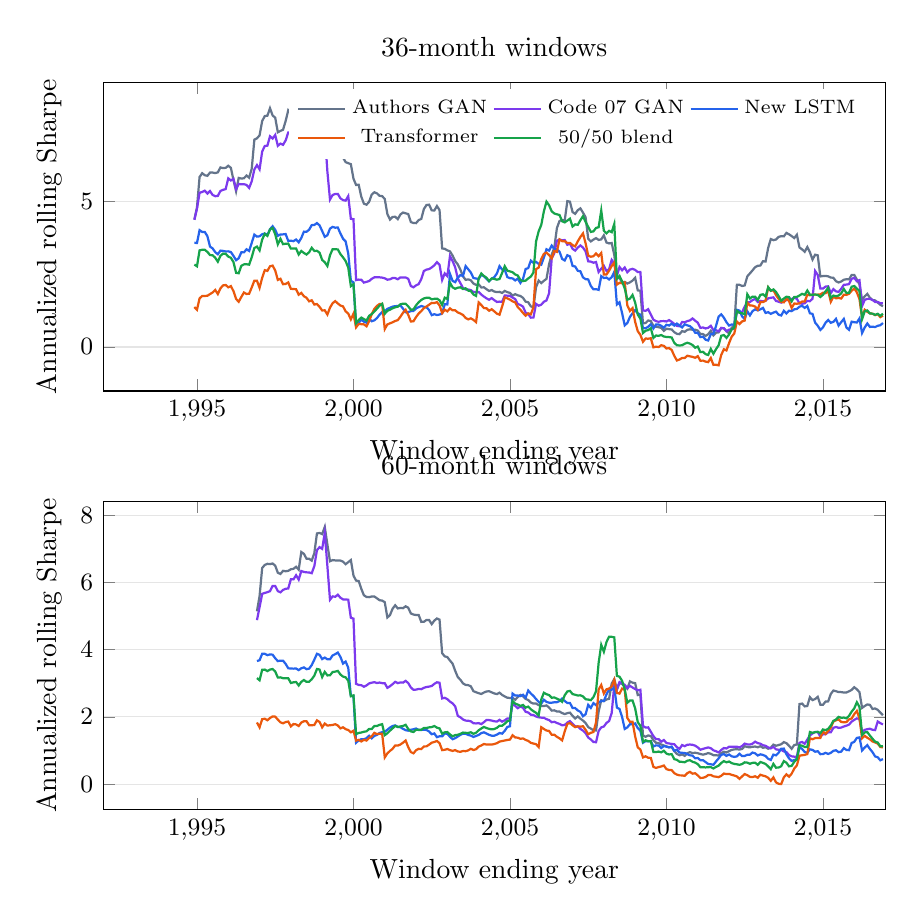
\begin{tikzpicture}
\begin{groupplot}[group style={group size=1 by 2,vertical sep=1.4cm},width=.95\linewidth,height=5.5cm,xmin=1992,xmax=2017,xtick={1995,2000,2005,2010,2015},ylabel={Annualized rolling Sharpe},ymajorgrids,grid style={gray!20},tick label style={font=\small},legend style={font=\scriptsize,draw=none},legend columns=3]
\nextgroupplot[title={36-month windows},xlabel={Window ending year}]
\addplot[papercolor,thick,no marks] coordinates {(1994.9167,4.362239) (1995.0000,4.779713) (1995.0833,5.824375) (1995.1667,5.954706) (1995.2500,5.884563) (1995.3333,5.864846) (1995.4167,5.975139) (1995.5000,5.975801) (1995.5833,5.958803) (1995.6667,5.983277) (1995.7500,6.151803) (1995.8333,6.128810) (1995.9167,6.138050) (1996.0000,6.209893) (1996.0833,6.138824) (1996.1667,5.717772) (1996.2500,5.335141) (1996.3333,5.793844) (1996.4167,5.771275) (1996.5000,5.781040) (1996.5833,5.874546) (1996.6667,5.801945) (1996.7500,6.109216) (1996.8333,7.103859) (1996.9167,7.150274) (1997.0000,7.250067) (1997.0833,7.741936) (1997.1667,7.912530) (1997.2500,7.924439) (1997.3333,8.181553) (1997.4167,7.932036) (1997.5000,7.856118) (1997.5833,7.357066) (1997.6667,7.404187) (1997.7500,7.442181) (1997.8333,7.744303) (1997.9167,8.114094) (1998.0000,8.019359) (1998.0833,7.965002) (1998.1667,7.941139) (1998.2500,7.832630) (1998.3333,7.999412) (1998.4167,7.889138) (1998.5000,7.563408) (1998.5833,7.393960) (1998.6667,7.264572) (1998.7500,7.324337) (1998.8333,7.061130) (1998.9167,7.063342) (1999.0000,6.933099) (1999.0833,6.943577) (1999.1667,6.747877) (1999.2500,6.609046) (1999.3333,6.586827) (1999.4167,6.602740) (1999.5000,6.562252) (1999.5833,6.561764) (1999.6667,6.488668) (1999.7500,6.332998) (1999.8333,6.298476) (1999.9167,6.263452) (2000.0000,5.768213) (2000.0833,5.552217) (2000.1667,5.557944) (2000.2500,5.149283) (2000.3333,4.910923) (2000.4167,4.874998) (2000.5000,4.974456) (2000.5833,5.222004) (2000.6667,5.300843) (2000.7500,5.264820) (2000.8333,5.180758) (2000.9167,5.168558) (2001.0000,5.069707) (2001.0833,4.556038) (2001.1667,4.367876) (2001.2500,4.455578) (2001.3333,4.460978) (2001.4167,4.381596) (2001.5000,4.541148) (2001.5833,4.606476) (2001.6667,4.580075) (2001.7500,4.554647) (2001.8333,4.281257) (2001.9167,4.247381) (2002.0000,4.243337) (2002.0833,4.346727) (2002.1667,4.388737) (2002.2500,4.727625) (2002.3333,4.865115) (2002.4167,4.875708) (2002.5000,4.682224) (2002.5833,4.675656) (2002.6667,4.829514) (2002.7500,4.689950) (2002.8333,3.376396) (2002.9167,3.362874) (2003.0000,3.310634) (2003.0833,3.276128) (2003.1667,3.131354) (2003.2500,2.941587) (2003.3333,2.830777) (2003.4167,2.646123) (2003.5000,2.420276) (2003.5833,2.300466) (2003.6667,2.315569) (2003.7500,2.284956) (2003.8333,2.172879) (2003.9167,2.128212) (2004.0000,2.146821) (2004.0833,2.040055) (2004.1667,2.044039) (2004.2500,1.979166) (2004.3333,1.919642) (2004.4167,1.949952) (2004.5000,1.898860) (2004.5833,1.879297) (2004.6667,1.888651) (2004.7500,1.850933) (2004.8333,1.921305) (2004.9167,1.878192) (2005.0000,1.852689) (2005.0833,1.759613) (2005.1667,1.809920) (2005.2500,1.770356) (2005.3333,1.747865) (2005.4167,1.683314) (2005.5000,1.553240) (2005.5833,1.531671) (2005.6667,1.392736) (2005.7500,1.355851) (2005.8333,2.047098) (2005.9167,2.274603) (2006.0000,2.189012) (2006.0833,2.267551) (2006.1667,2.333616) (2006.2500,2.837831) (2006.3333,3.162969) (2006.4167,3.400256) (2006.5000,4.073917) (2006.5833,4.318488) (2006.6667,4.347502) (2006.7500,4.340599) (2006.8333,4.998293) (2006.9167,4.977963) (2007.0000,4.624095) (2007.0833,4.562064) (2007.1667,4.686246) (2007.2500,4.748368) (2007.3333,4.604879) (2007.4167,4.444746) (2007.5000,3.708452) (2007.5833,3.616285) (2007.6667,3.679629) (2007.7500,3.730220) (2007.8333,3.669080) (2007.9167,3.686552) (2008.0000,3.825475) (2008.0833,3.578536) (2008.1667,3.548116) (2008.2500,3.563648) (2008.3333,3.150178) (2008.4167,2.347800) (2008.5000,2.369558) (2008.5833,2.203855) (2008.6667,2.231404) (2008.7500,2.174028) (2008.8333,2.214328) (2008.9167,2.275783) (2009.0000,2.368668) (2009.0833,1.938936) (2009.1667,1.925103) (2009.2500,0.808866) (2009.3333,0.821896) (2009.4167,0.907263) (2009.5000,0.888894) (2009.5833,0.723323) (2009.6667,0.691259) (2009.7500,0.676980) (2009.8333,0.654613) (2009.9167,0.553600) (2010.0000,0.625253) (2010.0833,0.609969) (2010.1667,0.599491) (2010.2500,0.507782) (2010.3333,0.450521) (2010.4167,0.439806) (2010.5000,0.542319) (2010.5833,0.518914) (2010.6667,0.587486) (2010.7500,0.605430) (2010.8333,0.590623) (2010.9167,0.593950) (2011.0000,0.562246) (2011.0833,0.448465) (2011.1667,0.441238) (2011.2500,0.377679) (2011.3333,0.437913) (2011.4167,0.553566) (2011.5000,0.399993) (2011.5833,0.489647) (2011.6667,0.500337) (2011.7500,0.652111) (2011.8333,0.637859) (2011.9167,0.542104) (2012.0000,0.465895) (2012.0833,0.662933) (2012.1667,0.717414) (2012.2500,2.129152) (2012.3333,2.130754) (2012.4167,2.089531) (2012.5000,2.107588) (2012.5833,2.421324) (2012.6667,2.521251) (2012.7500,2.624779) (2012.8333,2.734473) (2012.9167,2.781916) (2013.0000,2.790362) (2013.0833,2.938127) (2013.1667,2.928575) (2013.2500,3.395998) (2013.3333,3.697257) (2013.4167,3.660273) (2013.5000,3.682326) (2013.5833,3.772334) (2013.6667,3.796299) (2013.7500,3.789718) (2013.8333,3.908672) (2013.9167,3.859325) (2014.0000,3.800052) (2014.0833,3.731857) (2014.1667,3.845203) (2014.2500,3.409461) (2014.3333,3.344995) (2014.4167,3.262208) (2014.5000,3.423586) (2014.5833,3.246700) (2014.6667,2.994950) (2014.7500,3.161278) (2014.8333,3.139947) (2014.9167,2.417451) (2015.0000,2.430591) (2015.0833,2.436523) (2015.1667,2.419723) (2015.2500,2.378865) (2015.3333,2.370593) (2015.4167,2.253078) (2015.5000,2.209844) (2015.5833,2.242777) (2015.6667,2.303735) (2015.7500,2.321248) (2015.8333,2.315497) (2015.9167,2.467646) (2016.0000,2.470238) (2016.0833,2.309230) (2016.1667,2.144999) (2016.2500,1.607431) (2016.3333,1.734037) (2016.4167,1.820587) (2016.5000,1.686755) (2016.5833,1.607901) (2016.6667,1.595848) (2016.7500,1.522491) (2016.8333,1.445714) (2016.9167,1.397658)};
\addplot[repcolor,thick,no marks] coordinates {(1994.9167,4.357715) (1995.0000,4.735714) (1995.0833,5.287312) (1995.1667,5.309568) (1995.2500,5.355878) (1995.3333,5.256645) (1995.4167,5.343322) (1995.5000,5.209606) (1995.5833,5.166202) (1995.6667,5.176112) (1995.7500,5.347106) (1995.8333,5.383773) (1995.9167,5.410342) (1996.0000,5.777224) (1996.0833,5.706142) (1996.1667,5.761945) (1996.2500,5.409638) (1996.3333,5.588965) (1996.4167,5.573735) (1996.5000,5.578625) (1996.5833,5.552783) (1996.6667,5.449904) (1996.7500,5.679696) (1996.8333,6.083052) (1996.9167,6.232959) (1997.0000,6.086516) (1997.0833,6.697798) (1997.1667,6.886786) (1997.2500,6.897820) (1997.3333,7.220082) (1997.4167,7.143403) (1997.5000,7.264650) (1997.5833,6.893543) (1997.6667,6.968799) (1997.7500,6.926959) (1997.8333,7.079447) (1997.9167,7.352947) (1998.0000,7.350474) (1998.0833,7.339899) (1998.1667,7.358810) (1998.2500,7.051988) (1998.3333,7.216736) (1998.4167,7.407096) (1998.5000,7.578686) (1998.5833,7.649368) (1998.6667,7.587372) (1998.7500,7.548799) (1998.8333,7.357140) (1998.9167,7.296915) (1999.0000,7.229344) (1999.0833,7.358325) (1999.1667,6.013257) (1999.2500,5.052976) (1999.3333,5.205610) (1999.4167,5.244057) (1999.5000,5.246149) (1999.5833,5.092011) (1999.6667,5.032335) (1999.7500,5.015331) (1999.8333,5.169575) (1999.9167,4.392120) (2000.0000,4.379742) (2000.0833,2.291764) (2000.1667,2.308901) (2000.2500,2.302822) (2000.3333,2.205933) (2000.4167,2.232187) (2000.5000,2.258920) (2000.5833,2.335126) (2000.6667,2.385768) (2000.7500,2.387621) (2000.8333,2.386563) (2000.9167,2.376425) (2001.0000,2.353242) (2001.0833,2.305282) (2001.1667,2.318545) (2001.2500,2.364853) (2001.3333,2.360596) (2001.4167,2.319929) (2001.5000,2.384560) (2001.5833,2.379876) (2001.6667,2.382942) (2001.7500,2.336522) (2001.8333,2.089065) (2001.9167,2.044071) (2002.0000,2.111893) (2002.0833,2.155655) (2002.1667,2.326189) (2002.2500,2.602942) (2002.3333,2.651608) (2002.4167,2.669166) (2002.5000,2.725295) (2002.5833,2.798815) (2002.6667,2.905782) (2002.7500,2.815823) (2002.8333,2.296907) (2002.9167,2.520328) (2003.0000,2.429368) (2003.0833,3.111962) (2003.1667,2.943559) (2003.2500,2.731023) (2003.3333,2.348463) (2003.4167,2.187540) (2003.5000,2.021725) (2003.5833,1.968683) (2003.6667,1.967561) (2003.7500,1.948620) (2003.8333,1.882636) (2003.9167,1.878596) (2004.0000,1.885571) (2004.0833,1.795919) (2004.1667,1.727483) (2004.2500,1.666345) (2004.3333,1.617980) (2004.4167,1.674341) (2004.5000,1.604245) (2004.5833,1.542371) (2004.6667,1.554880) (2004.7500,1.546501) (2004.8333,1.763635) (2004.9167,1.758332) (2005.0000,1.748987) (2005.0833,1.693221) (2005.1667,1.641708) (2005.2500,1.470138) (2005.3333,1.439104) (2005.4167,1.382081) (2005.5000,1.175960) (2005.5833,1.127393) (2005.6667,1.004799) (2005.7500,1.006781) (2005.8333,1.475998) (2005.9167,1.414249) (2006.0000,1.449824) (2006.0833,1.547969) (2006.1667,1.595372) (2006.2500,1.842578) (2006.3333,3.033092) (2006.4167,3.211722) (2006.5000,3.637597) (2006.5833,3.680886) (2006.6667,3.655123) (2006.7500,3.666382) (2006.8333,3.502294) (2006.9167,3.538742) (2007.0000,3.364607) (2007.0833,3.301799) (2007.1667,3.404966) (2007.2500,3.479064) (2007.3333,3.407304) (2007.4167,3.274644) (2007.5000,2.933793) (2007.5833,2.924306) (2007.6667,2.887609) (2007.7500,2.909916) (2007.8333,2.567363) (2007.9167,2.682259) (2008.0000,2.779682) (2008.0833,2.604718) (2008.1667,2.665363) (2008.2500,2.983379) (2008.3333,2.862288) (2008.4167,2.439761) (2008.5000,2.739884) (2008.5833,2.627514) (2008.6667,2.722029) (2008.7500,2.558922) (2008.8333,2.652785) (2008.9167,2.677222) (2009.0000,2.639896) (2009.0833,2.566405) (2009.1667,2.570828) (2009.2500,1.251504) (2009.3333,1.238854) (2009.4167,1.293850) (2009.5000,1.116300) (2009.5833,0.934465) (2009.6667,0.884277) (2009.7500,0.861387) (2009.8333,0.885886) (2009.9167,0.886428) (2010.0000,0.874032) (2010.0833,0.921617) (2010.1667,0.860717) (2010.2500,0.790175) (2010.3333,0.722411) (2010.4167,0.709293) (2010.5000,0.855246) (2010.5833,0.847424) (2010.6667,0.886420) (2010.7500,0.910479) (2010.8333,0.977857) (2010.9167,0.900647) (2011.0000,0.833862) (2011.0833,0.655102) (2011.1667,0.668528) (2011.2500,0.634473) (2011.3333,0.657158) (2011.4167,0.725226) (2011.5000,0.576520) (2011.5833,0.573962) (2011.6667,0.536099) (2011.7500,0.649009) (2011.8333,0.644403) (2011.9167,0.541430) (2012.0000,0.593823) (2012.0833,0.603848) (2012.1667,0.632959) (2012.2500,1.206279) (2012.3333,1.196271) (2012.4167,1.190138) (2012.5000,1.383721) (2012.5833,1.526674) (2012.6667,1.540330) (2012.7500,1.605741) (2012.8333,1.648954) (2012.9167,1.541396) (2013.0000,1.579571) (2013.0833,1.565092) (2013.1667,1.587870) (2013.2500,1.665657) (2013.3333,1.684397) (2013.4167,1.700196) (2013.5000,1.578013) (2013.5833,1.548374) (2013.6667,1.519155) (2013.7500,1.562443) (2013.8333,1.607609) (2013.9167,1.654429) (2014.0000,1.638101) (2014.0833,1.694042) (2014.1667,1.649061) (2014.2500,1.492956) (2014.3333,1.482038) (2014.4167,1.497084) (2014.5000,1.579351) (2014.5833,1.566737) (2014.6667,1.654968) (2014.7500,2.601840) (2014.8333,2.468661) (2014.9167,2.001420) (2015.0000,2.001028) (2015.0833,2.068764) (2015.1667,2.078442) (2015.2500,1.844341) (2015.3333,1.982642) (2015.4167,1.904396) (2015.5000,1.888352) (2015.5833,1.992916) (2015.6667,2.128536) (2015.7500,2.137877) (2015.8333,2.154703) (2015.9167,2.333893) (2016.0000,2.369313) (2016.0833,2.253321) (2016.1667,2.290660) (2016.2500,1.403438) (2016.3333,1.612213) (2016.4167,1.648367) (2016.5000,1.648044) (2016.5833,1.612615) (2016.6667,1.544087) (2016.7500,1.540768) (2016.8333,1.501704) (2016.9167,1.498523)};
\addplot[lstmcolor,thick,no marks] coordinates {(1994.9167,3.570058) (1995.0000,3.563256) (1995.0833,4.002841) (1995.1667,3.942814) (1995.2500,3.940633) (1995.3333,3.795571) (1995.4167,3.439929) (1995.5000,3.378540) (1995.5833,3.248724) (1995.6667,3.176853) (1995.7500,3.301521) (1995.8333,3.291314) (1995.9167,3.273932) (1996.0000,3.276650) (1996.0833,3.251829) (1996.1667,3.120437) (1996.2500,2.974185) (1996.3333,3.039974) (1996.4167,3.242721) (1996.5000,3.241657) (1996.5833,3.347596) (1996.6667,3.291429) (1996.7500,3.570041) (1996.8333,3.850680) (1996.9167,3.781344) (1997.0000,3.792634) (1997.0833,3.862831) (1997.1667,3.888258) (1997.2500,3.834765) (1997.3333,4.036220) (1997.4167,4.137185) (1997.5000,4.014144) (1997.5833,3.809642) (1997.6667,3.856836) (1997.7500,3.857714) (1997.8333,3.868980) (1997.9167,3.632722) (1998.0000,3.641726) (1998.0833,3.625965) (1998.1667,3.681524) (1998.2500,3.584978) (1998.3333,3.735459) (1998.4167,3.951580) (1998.5000,3.945734) (1998.5833,4.018849) (1998.6667,4.174987) (1998.7500,4.182242) (1998.8333,4.244674) (1998.9167,4.167375) (1999.0000,3.973483) (1999.0833,3.775334) (1999.1667,3.828631) (1999.2500,4.055430) (1999.3333,4.114425) (1999.4167,4.087730) (1999.5000,4.092986) (1999.5833,3.886713) (1999.6667,3.708636) (1999.7500,3.617132) (1999.8333,3.202599) (1999.9167,2.271631) (2000.0000,2.214267) (2000.0833,0.729685) (2000.1667,0.824586) (2000.2500,0.938416) (2000.3333,0.865815) (2000.4167,0.831928) (2000.5000,0.969285) (2000.5833,0.881674) (2000.6667,0.912494) (2000.7500,0.990274) (2000.8333,1.106190) (2000.9167,1.196500) (2001.0000,1.219776) (2001.0833,1.304982) (2001.1667,1.341983) (2001.2500,1.382663) (2001.3333,1.399137) (2001.4167,1.402063) (2001.5000,1.422917) (2001.5833,1.314370) (2001.6667,1.187083) (2001.7500,1.196280) (2001.8333,1.227626) (2001.9167,1.233835) (2002.0000,1.321407) (2002.0833,1.364270) (2002.1667,1.403643) (2002.2500,1.375798) (2002.3333,1.363509) (2002.4167,1.264341) (2002.5000,1.090246) (2002.5833,1.122950) (2002.6667,1.095113) (2002.7500,1.110087) (2002.8333,1.150393) (2002.9167,1.462551) (2003.0000,1.457806) (2003.0833,2.505381) (2003.1667,2.267001) (2003.2500,2.222180) (2003.3333,2.373658) (2003.4167,2.463660) (2003.5000,2.431437) (2003.5833,2.770880) (2003.6667,2.662995) (2003.7500,2.553857) (2003.8333,2.363987) (2003.9167,2.346297) (2004.0000,2.326576) (2004.0833,2.468561) (2004.1667,2.427040) (2004.2500,2.338345) (2004.3333,2.249916) (2004.4167,2.340416) (2004.5000,2.393415) (2004.5833,2.520386) (2004.6667,2.770209) (2004.7500,2.653174) (2004.8333,2.643962) (2004.9167,2.394542) (2005.0000,2.356299) (2005.0833,2.349737) (2005.1667,2.281104) (2005.2500,2.341978) (2005.3333,2.192829) (2005.4167,2.331363) (2005.5000,2.670722) (2005.5833,2.703210) (2005.6667,2.959230) (2005.7500,2.882578) (2005.8333,2.917269) (2005.9167,2.845211) (2006.0000,2.818729) (2006.0833,3.063963) (2006.1667,3.348793) (2006.2500,3.301981) (2006.3333,3.474103) (2006.4167,3.355594) (2006.5000,3.344124) (2006.5833,3.265200) (2006.6667,3.018529) (2006.7500,2.963073) (2006.8333,3.143284) (2006.9167,3.103485) (2007.0000,2.778232) (2007.0833,2.756546) (2007.1667,2.610327) (2007.2500,2.592925) (2007.3333,2.383660) (2007.4167,2.323777) (2007.5000,2.315298) (2007.5833,2.092045) (2007.6667,1.974613) (2007.7500,1.981270) (2007.8333,1.956482) (2007.9167,2.426567) (2008.0000,2.362158) (2008.0833,2.378452) (2008.1667,2.313779) (2008.2500,2.390366) (2008.3333,2.573734) (2008.4167,1.456117) (2008.5000,1.531150) (2008.5833,1.156522) (2008.6667,0.741180) (2008.7500,0.821734) (2008.8333,1.029605) (2008.9167,1.154702) (2009.0000,1.263802) (2009.0833,1.151354) (2009.1667,1.107524) (2009.2500,0.645575) (2009.3333,0.641836) (2009.4167,0.694474) (2009.5000,0.778426) (2009.5833,0.632963) (2009.6667,0.770106) (2009.7500,0.768078) (2009.8333,0.727683) (2009.9167,0.656416) (2010.0000,0.760643) (2010.0833,0.734219) (2010.1667,0.795291) (2010.2500,0.734128) (2010.3333,0.801901) (2010.4167,0.735470) (2010.5000,0.670814) (2010.5833,0.776600) (2010.6667,0.740984) (2010.7500,0.712200) (2010.8333,0.635820) (2010.9167,0.489400) (2011.0000,0.486823) (2011.0833,0.338755) (2011.1667,0.353558) (2011.2500,0.249260) (2011.3333,0.221983) (2011.4167,0.441277) (2011.5000,0.451078) (2011.5833,0.718271) (2011.6667,1.039820) (2011.7500,1.117792) (2011.8333,1.004906) (2011.9167,0.850198) (2012.0000,0.733213) (2012.0833,0.771392) (2012.1667,0.753843) (2012.2500,1.273432) (2012.3333,1.245067) (2012.4167,1.049539) (2012.5000,0.956343) (2012.5833,1.225702) (2012.6667,1.082746) (2012.7500,1.228319) (2012.8333,1.289580) (2012.9167,1.254495) (2013.0000,1.289382) (2013.0833,1.339006) (2013.1667,1.166337) (2013.2500,1.191696) (2013.3333,1.135230) (2013.4167,1.176896) (2013.5000,1.211129) (2013.5833,1.106976) (2013.6667,1.079269) (2013.7500,1.237848) (2013.8333,1.147991) (2013.9167,1.242288) (2014.0000,1.227955) (2014.0833,1.290193) (2014.1667,1.304028) (2014.2500,1.380165) (2014.3333,1.410780) (2014.4167,1.339735) (2014.5000,1.405658) (2014.5833,1.154701) (2014.6667,1.133156) (2014.7500,0.834776) (2014.8333,0.727901) (2014.9167,0.585317) (2015.0000,0.669997) (2015.0833,0.832623) (2015.1667,0.924802) (2015.2500,0.829883) (2015.3333,0.860850) (2015.4167,0.963190) (2015.5000,0.732663) (2015.5833,0.851709) (2015.6667,0.961980) (2015.7500,0.664850) (2015.8333,0.588443) (2015.9167,0.866532) (2016.0000,0.847788) (2016.0833,0.838685) (2016.1667,0.977795) (2016.2500,0.478545) (2016.3333,0.665104) (2016.4167,0.805364) (2016.5000,0.687028) (2016.5833,0.695343) (2016.6667,0.682736) (2016.7500,0.726190) (2016.8333,0.744561) (2016.9167,0.820254)};
\addplot[transcolor,thick,no marks] coordinates {(1994.9167,1.366842) (1995.0000,1.275965) (1995.0833,1.666665) (1995.1667,1.746141) (1995.2500,1.747498) (1995.3333,1.755528) (1995.4167,1.812324) (1995.5000,1.868293) (1995.5833,1.954262) (1995.6667,1.814445) (1995.7500,2.008398) (1995.8333,2.109810) (1995.9167,2.124770) (1996.0000,2.043672) (1996.0833,2.085349) (1996.1667,1.912351) (1996.2500,1.645614) (1996.3333,1.549533) (1996.4167,1.712770) (1996.5000,1.865856) (1996.5833,1.816691) (1996.6667,1.824108) (1996.7500,2.041113) (1996.8333,2.272350) (1996.9167,2.268715) (1997.0000,2.026199) (1997.0833,2.371601) (1997.1667,2.631948) (1997.2500,2.606780) (1997.3333,2.764453) (1997.4167,2.788026) (1997.5000,2.621113) (1997.5833,2.297394) (1997.6667,2.336165) (1997.7500,2.151329) (1997.8333,2.159563) (1997.9167,2.213104) (1998.0000,1.993229) (1998.0833,1.985884) (1998.1667,1.978721) (1998.2500,1.791452) (1998.3333,1.852667) (1998.4167,1.737944) (1998.5000,1.685182) (1998.5833,1.564125) (1998.6667,1.599508) (1998.7500,1.452831) (1998.8333,1.471865) (1998.9167,1.374351) (1999.0000,1.251787) (1999.0833,1.256375) (1999.1667,1.110476) (1999.2500,1.347336) (1999.3333,1.498370) (1999.4167,1.570581) (1999.5000,1.490935) (1999.5833,1.420460) (1999.6667,1.390046) (1999.7500,1.220257) (1999.8333,1.145892) (1999.9167,0.944974) (2000.0000,1.140076) (2000.0833,0.672178) (2000.1667,0.790867) (2000.2500,0.781254) (2000.3333,0.774471) (2000.4167,0.708879) (2000.5000,0.884343) (2000.5833,1.124076) (2000.6667,1.305060) (2000.7500,1.407486) (2000.8333,1.472869) (2000.9167,1.474443) (2001.0000,0.614212) (2001.0833,0.772802) (2001.1667,0.809432) (2001.2500,0.846690) (2001.3333,0.891493) (2001.4167,0.919600) (2001.5000,1.037231) (2001.5833,1.172614) (2001.6667,1.272460) (2001.7500,1.100528) (2001.8333,0.872270) (2001.9167,0.881639) (2002.0000,1.025919) (2002.0833,1.146217) (2002.1667,1.230302) (2002.2500,1.330858) (2002.3333,1.385549) (2002.4167,1.449290) (2002.5000,1.511568) (2002.5833,1.504377) (2002.6667,1.536968) (2002.7500,1.426074) (2002.8333,1.159004) (2002.9167,1.276641) (2003.0000,1.220454) (2003.0833,1.322112) (2003.1667,1.254590) (2003.2500,1.255964) (2003.3333,1.183424) (2003.4167,1.146075) (2003.5000,1.096094) (2003.5833,0.994703) (2003.6667,0.945521) (2003.7500,0.980522) (2003.8333,0.927657) (2003.9167,0.851567) (2004.0000,1.525438) (2004.0833,1.439234) (2004.1667,1.332801) (2004.2500,1.326757) (2004.3333,1.240611) (2004.4167,1.292789) (2004.5000,1.219407) (2004.5833,1.141857) (2004.6667,1.105950) (2004.7500,1.387647) (2004.8333,1.697560) (2004.9167,1.665680) (2005.0000,1.623076) (2005.0833,1.562196) (2005.1667,1.527478) (2005.2500,1.364948) (2005.3333,1.276405) (2005.4167,1.166970) (2005.5000,1.071893) (2005.5833,1.151964) (2005.6667,1.118885) (2005.7500,1.357512) (2005.8333,2.667060) (2005.9167,2.720762) (2006.0000,3.015966) (2006.0833,3.192297) (2006.1667,3.231137) (2006.2500,3.149264) (2006.3333,3.039770) (2006.4167,3.289599) (2006.5000,3.260170) (2006.5833,3.683804) (2006.6667,3.625832) (2006.7500,3.626036) (2006.8333,3.560388) (2006.9167,3.566501) (2007.0000,3.492596) (2007.0833,3.447251) (2007.1667,3.620228) (2007.2500,3.768818) (2007.3333,3.891101) (2007.4167,3.551387) (2007.5000,3.131895) (2007.5833,3.091392) (2007.6667,3.110392) (2007.7500,3.203225) (2007.8333,3.113338) (2007.9167,3.220334) (2008.0000,2.483906) (2008.0833,2.483901) (2008.1667,2.610851) (2008.2500,2.774214) (2008.3333,2.895753) (2008.4167,2.136468) (2008.5000,2.198665) (2008.5833,2.182612) (2008.6667,2.208786) (2008.7500,1.424541) (2008.8333,1.234085) (2008.9167,1.329489) (2009.0000,0.857980) (2009.0833,0.539912) (2009.1667,0.416790) (2009.2500,0.177887) (2009.3333,0.289235) (2009.4167,0.283274) (2009.5000,0.299571) (2009.5833,-0.011608) (2009.6667,0.009384) (2009.7500,-0.001478) (2009.8333,0.059713) (2009.9167,0.037280) (2010.0000,-0.052135) (2010.0833,-0.038740) (2010.1667,-0.101383) (2010.2500,-0.303194) (2010.3333,-0.462711) (2010.4167,-0.430060) (2010.5000,-0.375418) (2010.5833,-0.377011) (2010.6667,-0.299806) (2010.7500,-0.321630) (2010.8333,-0.338480) (2010.9167,-0.370610) (2011.0000,-0.315002) (2011.0833,-0.470462) (2011.1667,-0.467152) (2011.2500,-0.501072) (2011.3333,-0.518074) (2011.4167,-0.378547) (2011.5000,-0.614139) (2011.5833,-0.610236) (2011.6667,-0.628124) (2011.7500,-0.273669) (2011.8333,-0.078776) (2011.9167,-0.118805) (2012.0000,0.130030) (2012.0833,0.351477) (2012.1667,0.461991) (2012.2500,0.868663) (2012.3333,0.785238) (2012.4167,0.876016) (2012.5000,0.905223) (2012.5833,1.519950) (2012.6667,1.420477) (2012.7500,1.417340) (2012.8333,1.383855) (2012.9167,1.278998) (2013.0000,1.542150) (2013.0833,1.537386) (2013.1667,1.583280) (2013.2500,2.038027) (2013.3333,1.924017) (2013.4167,1.948342) (2013.5000,1.773101) (2013.5833,1.651690) (2013.6667,1.541460) (2013.7500,1.528955) (2013.8333,1.658647) (2013.9167,1.574847) (2014.0000,1.338252) (2014.0833,1.489624) (2014.1667,1.480577) (2014.2500,1.497354) (2014.3333,1.556635) (2014.4167,1.557098) (2014.5000,1.787983) (2014.5833,1.770920) (2014.6667,1.792364) (2014.7500,1.793486) (2014.8333,1.793641) (2014.9167,1.798161) (2015.0000,1.858857) (2015.0833,1.844219) (2015.1667,1.926070) (2015.2500,1.549116) (2015.3333,1.720699) (2015.4167,1.666742) (2015.5000,1.679054) (2015.5833,1.659248) (2015.6667,1.789442) (2015.7500,1.784458) (2015.8333,1.823314) (2015.9167,1.927133) (2016.0000,2.002283) (2016.0833,1.871517) (2016.1667,1.639686) (2016.2500,0.999905) (2016.3333,1.274993) (2016.4167,1.205346) (2016.5000,1.152741) (2016.5833,1.139039) (2016.6667,1.092614) (2016.7500,1.121164) (2016.8333,1.022736) (2016.9167,1.071844)};
\addplot[blendcolor,thick,no marks] coordinates {(1994.9167,2.823120) (1995.0000,2.765217) (1995.0833,3.311445) (1995.1667,3.330674) (1995.2500,3.329169) (1995.3333,3.257451) (1995.4167,3.149803) (1995.5000,3.140979) (1995.5833,3.057823) (1995.6667,2.922854) (1995.7500,3.123079) (1995.8333,3.199852) (1995.9167,3.192126) (1996.0000,3.098038) (1996.0833,3.055997) (1996.1667,2.907445) (1996.2500,2.541248) (1996.3333,2.525652) (1996.4167,2.779794) (1996.5000,2.830282) (1996.5833,2.834918) (1996.6667,2.820237) (1996.7500,3.078149) (1996.8333,3.392585) (1996.9167,3.439096) (1997.0000,3.307592) (1997.0833,3.681575) (1997.1667,3.876306) (1997.2500,3.806627) (1997.3333,4.027892) (1997.4167,4.078475) (1997.5000,3.862041) (1997.5833,3.517870) (1997.6667,3.706521) (1997.7500,3.523774) (1997.8333,3.538052) (1997.9167,3.542604) (1998.0000,3.369931) (1998.0833,3.371206) (1998.1667,3.376117) (1998.2500,3.169113) (1998.3333,3.289103) (1998.4167,3.220488) (1998.5000,3.167972) (1998.5833,3.245745) (1998.6667,3.398471) (1998.7500,3.289466) (1998.8333,3.295167) (1998.9167,3.230901) (1999.0000,2.982877) (1999.0833,2.902866) (1999.1667,2.773599) (1999.2500,3.142398) (1999.3333,3.349760) (1999.4167,3.348623) (1999.5000,3.342246) (1999.5833,3.181894) (1999.6667,3.070985) (1999.7500,2.942682) (1999.8333,2.719832) (1999.9167,2.084826) (2000.0000,2.151002) (2000.0833,0.817688) (2000.1667,0.923561) (2000.2500,1.007077) (2000.3333,0.956391) (2000.4167,0.904752) (2000.5000,1.067673) (2000.5833,1.127129) (2000.6667,1.213814) (2000.7500,1.312057) (2000.8333,1.416405) (2000.9167,1.479545) (2001.0000,1.138541) (2001.0833,1.238387) (2001.1667,1.278035) (2001.2500,1.325938) (2001.3333,1.361027) (2001.4167,1.380612) (2001.5000,1.464453) (2001.5833,1.482635) (2001.6667,1.479787) (2001.7500,1.391063) (2001.8333,1.275992) (2001.9167,1.285650) (2002.0000,1.427182) (2002.0833,1.532039) (2002.1667,1.611579) (2002.2500,1.663367) (2002.3333,1.688456) (2002.4167,1.687861) (2002.5000,1.632470) (2002.5833,1.649580) (2002.6667,1.656913) (2002.7500,1.600620) (2002.8333,1.441857) (2002.9167,1.689136) (2003.0000,1.645758) (2003.0833,2.200901) (2003.1667,2.043628) (2003.2500,1.994749) (2003.3333,2.030236) (2003.4167,2.045360) (2003.5000,1.985415) (2003.5833,2.011909) (2003.6667,1.930754) (2003.7500,1.914306) (2003.8333,1.799331) (2003.9167,1.750583) (2004.0000,2.347339) (2004.0833,2.516993) (2004.1667,2.432601) (2004.2500,2.372025) (2004.3333,2.258555) (2004.4167,2.348161) (2004.5000,2.331564) (2004.5833,2.305427) (2004.6667,2.328812) (2004.7500,2.538895) (2004.8333,2.768015) (2004.9167,2.613560) (2005.0000,2.589520) (2005.0833,2.560441) (2005.1667,2.485628) (2005.2500,2.448351) (2005.3333,2.295499) (2005.4167,2.256971) (2005.5000,2.273829) (2005.5833,2.347803) (2005.6667,2.412549) (2005.7500,2.550039) (2005.8333,3.613928) (2005.9167,3.963447) (2006.0000,4.180673) (2006.0833,4.648246) (2006.1667,4.980399) (2006.2500,4.856595) (2006.3333,4.648819) (2006.4167,4.575039) (2006.5000,4.545996) (2006.5833,4.522557) (2006.6667,4.306889) (2006.7500,4.269861) (2006.8333,4.332177) (2006.9167,4.395696) (2007.0000,4.127714) (2007.0833,4.201630) (2007.1667,4.185529) (2007.2500,4.343056) (2007.3333,4.481954) (2007.4167,4.285102) (2007.5000,4.113887) (2007.5833,3.944286) (2007.6667,3.960418) (2007.7500,4.078825) (2007.8333,4.102426) (2007.9167,4.674516) (2008.0000,3.982671) (2008.0833,3.893859) (2008.1667,3.978562) (2008.2500,3.932132) (2008.3333,4.216088) (2008.4167,2.341014) (2008.5000,2.433519) (2008.5833,2.244582) (2008.6667,2.007760) (2008.7500,1.618277) (2008.8333,1.655978) (2008.9167,1.783194) (2009.0000,1.521592) (2009.0833,1.109060) (2009.1667,0.971676) (2009.2500,0.478491) (2009.3333,0.555978) (2009.4167,0.579716) (2009.5000,0.641428) (2009.5833,0.308968) (2009.6667,0.392101) (2009.7500,0.383443) (2009.8333,0.408270) (2009.9167,0.358567) (2010.0000,0.342418) (2010.0833,0.338520) (2010.1667,0.323869) (2010.2500,0.141423) (2010.3333,0.059452) (2010.4167,0.051294) (2010.5000,0.058892) (2010.5833,0.110700) (2010.6667,0.144828) (2010.7500,0.116353) (2010.8333,0.065727) (2010.9167,-0.026685) (2011.0000,0.015190) (2011.0833,-0.175608) (2011.1667,-0.165504) (2011.2500,-0.246764) (2011.3333,-0.273631) (2011.4167,-0.068624) (2011.5000,-0.230757) (2011.5833,-0.073613) (2011.6667,0.058242) (2011.7500,0.382942) (2011.8333,0.409797) (2011.9167,0.311846) (2012.0000,0.424763) (2012.0833,0.600815) (2012.1667,0.667180) (2012.2500,1.237451) (2012.3333,1.170541) (2012.4167,1.155378) (2012.5000,1.118039) (2012.5833,1.805790) (2012.6667,1.661425) (2012.7500,1.725251) (2012.8333,1.721044) (2012.9167,1.610708) (2013.0000,1.783671) (2013.0833,1.805558) (2013.1667,1.725894) (2013.2500,2.048771) (2013.3333,1.927116) (2013.4167,1.971550) (2013.5000,1.884513) (2013.5833,1.743912) (2013.6667,1.583039) (2013.7500,1.659473) (2013.8333,1.721223) (2013.9167,1.707777) (2014.0000,1.563684) (2014.0833,1.713648) (2014.1667,1.714404) (2014.2500,1.764447) (2014.3333,1.822187) (2014.4167,1.785340) (2014.5000,1.934577) (2014.5833,1.792446) (2014.6667,1.787215) (2014.7500,1.798512) (2014.8333,1.784496) (2014.9167,1.712760) (2015.0000,1.787719) (2015.0833,1.907824) (2015.1667,2.026021) (2015.2500,1.674945) (2015.3333,1.761410) (2015.4167,1.739521) (2015.5000,1.761955) (2015.5833,1.837846) (2015.6667,1.988003) (2015.7500,1.849709) (2015.8333,1.857824) (2015.9167,2.065776) (2016.0000,2.087604) (2016.0833,2.001466) (2016.1667,1.913615) (2016.2500,0.957732) (2016.3333,1.222009) (2016.4167,1.252054) (2016.5000,1.147187) (2016.5833,1.142193) (2016.6667,1.099723) (2016.7500,1.137391) (2016.8333,1.067562) (2016.9167,1.139103)};\legend{Authors GAN,Code 07 GAN,New LSTM,Transformer,50/50 blend}
\nextgroupplot[title={60-month windows},xlabel={Window ending year}]
\addplot[papercolor,thick,no marks] coordinates {(1996.9167,5.140653) (1997.0000,5.591894) (1997.0833,6.429481) (1997.1667,6.518499) (1997.2500,6.552249) (1997.3333,6.542759) (1997.4167,6.562644) (1997.5000,6.496417) (1997.5833,6.286597) (1997.6667,6.250505) (1997.7500,6.343890) (1997.8333,6.330993) (1997.9167,6.344332) (1998.0000,6.390200) (1998.0833,6.403624) (1998.1667,6.464952) (1998.2500,6.378767) (1998.3333,6.903102) (1998.4167,6.848964) (1998.5000,6.705502) (1998.5833,6.703716) (1998.6667,6.645956) (1998.7500,6.873627) (1998.8333,7.454621) (1998.9167,7.470165) (1999.0000,7.435708) (1999.0833,7.648262) (1999.1667,7.125867) (1999.2500,6.630033) (1999.3333,6.662975) (1999.4167,6.653889) (1999.5000,6.650090) (1999.5833,6.647978) (1999.6667,6.616519) (1999.7500,6.540713) (1999.8333,6.602566) (1999.9167,6.664382) (2000.0000,6.204213) (2000.0833,6.053642) (2000.1667,6.040052) (2000.2500,5.807907) (2000.3333,5.617274) (2000.4167,5.567218) (2000.5000,5.560801) (2000.5833,5.580461) (2000.6667,5.580375) (2000.7500,5.527277) (2000.8333,5.469944) (2000.9167,5.458997) (2001.0000,5.410237) (2001.0833,4.955930) (2001.1667,5.027861) (2001.2500,5.217488) (2001.3333,5.319093) (2001.4167,5.224953) (2001.5000,5.242068) (2001.5833,5.232532) (2001.6667,5.289040) (2001.7500,5.246653) (2001.8333,5.076281) (2001.9167,5.043633) (2002.0000,5.031101) (2002.0833,5.031333) (2002.1667,4.825629) (2002.2500,4.828729) (2002.3333,4.882349) (2002.4167,4.881363) (2002.5000,4.758053) (2002.5833,4.863687) (2002.6667,4.926995) (2002.7500,4.892386) (2002.8333,3.893811) (2002.9167,3.799908) (2003.0000,3.778211) (2003.0833,3.675449) (2003.1667,3.583543) (2003.2500,3.371140) (2003.3333,3.184822) (2003.4167,3.104390) (2003.5000,2.995950) (2003.5833,2.951842) (2003.6667,2.944586) (2003.7500,2.908336) (2003.8333,2.765218) (2003.9167,2.733062) (2004.0000,2.705676) (2004.0833,2.681847) (2004.1667,2.724272) (2004.2500,2.756034) (2004.3333,2.764224) (2004.4167,2.729976) (2004.5000,2.697390) (2004.5833,2.678790) (2004.6667,2.721192) (2004.7500,2.652265) (2004.8333,2.609801) (2004.9167,2.571243) (2005.0000,2.562290) (2005.0833,2.567240) (2005.1667,2.508555) (2005.2500,2.591592) (2005.3333,2.654063) (2005.4167,2.611060) (2005.5000,2.535523) (2005.5833,2.501911) (2005.6667,2.427720) (2005.7500,2.395441) (2005.8333,2.396757) (2005.9167,2.350642) (2006.0000,2.324795) (2006.0833,2.322724) (2006.1667,2.341980) (2006.2500,2.278239) (2006.3333,2.187234) (2006.4167,2.196044) (2006.5000,2.160969) (2006.5833,2.159819) (2006.6667,2.113036) (2006.7500,2.086317) (2006.8333,2.111912) (2006.9167,2.126990) (2007.0000,2.031127) (2007.0833,1.954456) (2007.1667,2.014303) (2007.2500,1.947412) (2007.3333,1.891324) (2007.4167,1.818206) (2007.5000,1.697741) (2007.5833,1.653176) (2007.6667,1.601857) (2007.7500,1.598152) (2007.8333,2.163204) (2007.9167,2.495964) (2008.0000,2.468365) (2008.0833,2.518047) (2008.1667,2.538155) (2008.2500,2.991092) (2008.3333,3.125312) (2008.4167,2.806371) (2008.5000,3.010143) (2008.5833,2.978592) (2008.6667,2.901377) (2008.7500,2.837374) (2008.8333,3.057783) (2008.9167,3.018507) (2009.0000,3.003057) (2009.0833,2.650278) (2009.1667,2.664030) (2009.2500,1.444208) (2009.3333,1.409021) (2009.4167,1.448895) (2009.5000,1.431455) (2009.5833,1.308404) (2009.6667,1.231765) (2009.7500,1.221610) (2009.8333,1.178803) (2009.9167,1.149961) (2010.0000,1.123265) (2010.0833,1.093704) (2010.1667,1.105531) (2010.2500,0.983094) (2010.3333,0.899330) (2010.4167,0.859604) (2010.5000,0.885605) (2010.5833,0.841642) (2010.6667,0.920230) (2010.7500,0.952033) (2010.8333,0.926431) (2010.9167,0.933897) (2011.0000,0.921487) (2011.0833,0.896099) (2011.1667,0.878013) (2011.2500,0.896508) (2011.3333,0.924804) (2011.4167,0.902971) (2011.5000,0.861250) (2011.5833,0.860248) (2011.6667,0.851891) (2011.7500,0.925235) (2011.8333,0.964706) (2011.9167,0.940662) (2012.0000,0.982995) (2012.0833,1.018100) (2012.1667,1.033883) (2012.2500,1.039031) (2012.3333,1.028790) (2012.4167,1.047666) (2012.5000,1.129920) (2012.5833,1.103434) (2012.6667,1.096359) (2012.7500,1.111103) (2012.8333,1.118953) (2012.9167,1.097522) (2013.0000,1.128863) (2013.0833,1.083222) (2013.1667,1.097429) (2013.2500,1.053766) (2013.3333,1.086084) (2013.4167,1.175693) (2013.5000,1.140944) (2013.5833,1.164648) (2013.6667,1.187232) (2013.7500,1.250227) (2013.8333,1.219132) (2013.9167,1.141247) (2014.0000,1.053070) (2014.0833,1.164435) (2014.1667,1.178349) (2014.2500,2.381630) (2014.3333,2.396590) (2014.4167,2.313124) (2014.5000,2.325418) (2014.5833,2.585597) (2014.6667,2.499599) (2014.7500,2.531334) (2014.8333,2.596292) (2014.9167,2.361958) (2015.0000,2.360685) (2015.0833,2.455732) (2015.1667,2.460886) (2015.2500,2.682137) (2015.3333,2.783875) (2015.4167,2.764312) (2015.5000,2.738483) (2015.5833,2.737384) (2015.6667,2.725202) (2015.7500,2.726657) (2015.8333,2.762195) (2015.9167,2.802476) (2016.0000,2.882571) (2016.0833,2.820910) (2016.1667,2.734850) (2016.2500,2.268765) (2016.3333,2.323393) (2016.4167,2.370472) (2016.5000,2.357382) (2016.5833,2.237547) (2016.6667,2.251256) (2016.7500,2.209953) (2016.8333,2.127233) (2016.9167,2.052465)};
\addplot[repcolor,thick,no marks] coordinates {(1996.9167,4.878645) (1997.0000,5.260617) (1997.0833,5.658811) (1997.1667,5.685887) (1997.2500,5.709410) (1997.3333,5.738971) (1997.4167,5.893734) (1997.5000,5.892276) (1997.5833,5.740771) (1997.6667,5.705163) (1997.7500,5.775575) (1997.8333,5.809740) (1997.9167,5.818902) (1998.0000,6.092247) (1998.0833,6.089589) (1998.1667,6.212491) (1998.2500,6.081901) (1998.3333,6.338120) (1998.4167,6.309633) (1998.5000,6.298653) (1998.5833,6.295016) (1998.6667,6.273020) (1998.7500,6.486470) (1998.8333,6.959178) (1998.9167,7.047101) (1999.0000,6.997071) (1999.0833,7.473602) (1999.1667,6.486919) (1999.2500,5.484389) (1999.3333,5.583363) (1999.4167,5.572503) (1999.5000,5.634558) (1999.5833,5.544283) (1999.6667,5.493470) (1999.7500,5.494116) (1999.8333,5.484111) (1999.9167,4.948288) (2000.0000,4.922514) (2000.0833,2.984013) (2000.1667,2.950787) (2000.2500,2.942794) (2000.3333,2.898042) (2000.4167,2.937048) (2000.5000,2.995444) (2000.5833,3.017589) (2000.6667,3.031962) (2000.7500,3.008548) (2000.8333,3.021855) (2000.9167,3.003855) (2001.0000,3.001210) (2001.0833,2.864086) (2001.1667,2.912890) (2001.2500,2.973827) (2001.3333,3.042966) (2001.4167,3.004022) (2001.5000,3.025915) (2001.5833,3.018982) (2001.6667,3.071202) (2001.7500,3.005983) (2001.8333,2.875904) (2001.9167,2.805166) (2002.0000,2.811671) (2002.0833,2.832944) (2002.1667,2.824032) (2002.2500,2.865143) (2002.3333,2.889499) (2002.4167,2.901268) (2002.5000,2.919623) (2002.5833,2.982707) (2002.6667,3.029705) (2002.7500,3.014899) (2002.8333,2.549255) (2002.9167,2.568068) (2003.0000,2.526853) (2003.0833,2.455718) (2003.1667,2.403001) (2003.2500,2.312893) (2003.3333,2.031287) (2003.4167,1.988440) (2003.5000,1.924181) (2003.5833,1.889823) (2003.6667,1.887125) (2003.7500,1.868101) (2003.8333,1.812434) (2003.9167,1.806069) (2004.0000,1.815553) (2004.0833,1.786094) (2004.1667,1.842844) (2004.2500,1.908345) (2004.3333,1.905267) (2004.4167,1.890818) (2004.5000,1.870143) (2004.5833,1.861180) (2004.6667,1.913076) (2004.7500,1.858305) (2004.8333,1.899321) (2004.9167,1.953259) (2005.0000,1.951982) (2005.0833,2.399758) (2005.1667,2.328738) (2005.2500,2.258590) (2005.3333,2.312187) (2005.4167,2.269632) (2005.5000,2.152171) (2005.5833,2.130660) (2005.6667,2.065836) (2005.7500,2.055035) (2005.8333,2.012147) (2005.9167,1.988157) (2006.0000,1.978338) (2006.0833,1.974244) (2006.1667,1.933190) (2006.2500,1.906818) (2006.3333,1.842138) (2006.4167,1.855033) (2006.5000,1.819088) (2006.5833,1.791015) (2006.6667,1.751398) (2006.7500,1.759511) (2006.8333,1.831741) (2006.9167,1.875950) (2007.0000,1.796486) (2007.0833,1.721895) (2007.1667,1.714172) (2007.2500,1.644470) (2007.3333,1.592189) (2007.4167,1.518184) (2007.5000,1.387960) (2007.5833,1.328839) (2007.6667,1.255584) (2007.7500,1.246605) (2007.8333,1.582286) (2007.9167,1.689621) (2008.0000,1.714761) (2008.0833,1.820266) (2008.1667,1.876890) (2008.2500,2.112533) (2008.3333,2.955491) (2008.4167,2.839357) (2008.5000,3.034787) (2008.5833,2.996510) (2008.6667,2.956055) (2008.7500,2.855980) (2008.8333,2.924506) (2008.9167,2.873576) (2009.0000,2.828452) (2009.0833,2.790945) (2009.1667,2.807473) (2009.2500,1.729961) (2009.3333,1.683173) (2009.4167,1.689321) (2009.5000,1.559618) (2009.5833,1.428353) (2009.6667,1.340148) (2009.7500,1.338438) (2009.8333,1.261827) (2009.9167,1.312792) (2010.0000,1.222922) (2010.0833,1.210390) (2010.1667,1.195864) (2010.2500,1.188125) (2010.3333,1.100176) (2010.4167,1.049594) (2010.5000,1.162823) (2010.5833,1.130212) (2010.6667,1.170920) (2010.7500,1.178433) (2010.8333,1.170781) (2010.9167,1.145336) (2011.0000,1.094662) (2011.0833,1.023304) (2011.1667,1.049598) (2011.2500,1.071403) (2011.3333,1.092800) (2011.4167,1.069693) (2011.5000,1.007725) (2011.5833,0.979340) (2011.6667,0.944016) (2011.7500,1.017320) (2011.8333,1.074857) (2011.9167,1.061780) (2012.0000,1.111499) (2012.0833,1.114870) (2012.1667,1.114382) (2012.2500,1.114994) (2012.3333,1.091787) (2012.4167,1.135454) (2012.5000,1.206158) (2012.5833,1.182832) (2012.6667,1.176649) (2012.7500,1.204702) (2012.8333,1.264030) (2012.9167,1.220573) (2013.0000,1.203981) (2013.0833,1.158616) (2013.1667,1.140691) (2013.2500,1.092133) (2013.3333,1.064965) (2013.4167,1.109784) (2013.5000,1.034862) (2013.5833,1.022100) (2013.6667,1.020312) (2013.7500,0.974145) (2013.8333,0.953929) (2013.9167,0.865310) (2014.0000,0.827658) (2014.0833,0.817247) (2014.1667,0.814968) (2014.2500,1.229850) (2014.3333,1.254863) (2014.4167,1.202409) (2014.5000,1.325004) (2014.5833,1.446575) (2014.6667,1.507744) (2014.7500,1.550821) (2014.8333,1.551484) (2014.9167,1.412644) (2015.0000,1.484343) (2015.0833,1.481717) (2015.1667,1.545878) (2015.2500,1.541720) (2015.3333,1.675671) (2015.4167,1.701130) (2015.5000,1.673419) (2015.5833,1.682931) (2015.6667,1.715494) (2015.7500,1.739127) (2015.8333,1.770719) (2015.9167,1.860279) (2016.0000,1.912770) (2016.0833,1.956709) (2016.1667,1.938626) (2016.2500,1.554106) (2016.3333,1.614499) (2016.4167,1.635621) (2016.5000,1.649058) (2016.5833,1.616740) (2016.6667,1.608472) (2016.7500,1.862928) (2016.8333,1.814390) (2016.9167,1.774590)};
\addplot[lstmcolor,thick,no marks] coordinates {(1996.9167,3.660035) (1997.0000,3.685563) (1997.0833,3.875262) (1997.1667,3.875578) (1997.2500,3.835672) (1997.3333,3.858872) (1997.4167,3.849657) (1997.5000,3.744103) (1997.5833,3.659667) (1997.6667,3.672177) (1997.7500,3.671369) (1997.8333,3.576710) (1997.9167,3.445803) (1998.0000,3.438363) (1998.0833,3.435172) (1998.1667,3.438894) (1998.2500,3.391876) (1998.3333,3.446420) (1998.4167,3.473111) (1998.5000,3.419959) (1998.5833,3.436330) (1998.6667,3.541415) (1998.7500,3.703872) (1998.8333,3.875976) (1998.9167,3.845219) (1999.0000,3.719139) (1999.0833,3.764333) (1999.1667,3.713804) (1999.2500,3.713207) (1999.3333,3.827413) (1999.4167,3.866315) (1999.5000,3.913295) (1999.5833,3.785177) (1999.6667,3.586730) (1999.7500,3.645443) (1999.8333,3.462381) (1999.9167,2.628808) (2000.0000,2.616414) (2000.0833,1.232819) (2000.1667,1.302012) (2000.2500,1.336825) (2000.3333,1.331693) (2000.4167,1.369135) (2000.5000,1.439948) (2000.5833,1.362124) (2000.6667,1.435544) (2000.7500,1.464146) (2000.8333,1.522082) (2000.9167,1.547060) (2001.0000,1.560056) (2001.0833,1.618593) (2001.1667,1.682776) (2001.2500,1.729293) (2001.3333,1.747170) (2001.4167,1.700812) (2001.5000,1.693159) (2001.5833,1.645296) (2001.6667,1.605140) (2001.7500,1.589777) (2001.8333,1.617780) (2001.9167,1.632964) (2002.0000,1.655319) (2002.0833,1.610967) (2002.1667,1.612211) (2002.2500,1.617505) (2002.3333,1.612042) (2002.4167,1.565822) (2002.5000,1.484883) (2002.5833,1.508753) (2002.6667,1.397263) (2002.7500,1.424130) (2002.8333,1.421193) (2002.9167,1.507160) (2003.0000,1.495825) (2003.0833,1.410803) (2003.1667,1.336333) (2003.2500,1.368404) (2003.3333,1.416975) (2003.4167,1.466725) (2003.5000,1.502797) (2003.5833,1.497573) (2003.6667,1.464507) (2003.7500,1.443802) (2003.8333,1.404437) (2003.9167,1.432681) (2004.0000,1.464230) (2004.0833,1.517504) (2004.1667,1.541937) (2004.2500,1.505825) (2004.3333,1.465952) (2004.4167,1.441209) (2004.5000,1.442136) (2004.5833,1.473760) (2004.6667,1.520004) (2004.7500,1.502457) (2004.8333,1.587399) (2004.9167,1.701428) (2005.0000,1.722195) (2005.0833,2.693656) (2005.1667,2.634427) (2005.2500,2.635950) (2005.3333,2.618415) (2005.4167,2.658281) (2005.5000,2.572245) (2005.5833,2.784244) (2005.6667,2.695801) (2005.7500,2.625190) (2005.8333,2.530801) (2005.9167,2.447655) (2006.0000,2.393724) (2006.0833,2.510817) (2006.1667,2.446652) (2006.2500,2.423813) (2006.3333,2.422141) (2006.4167,2.435496) (2006.5000,2.437881) (2006.5833,2.470913) (2006.6667,2.546477) (2006.7500,2.472098) (2006.8333,2.414603) (2006.9167,2.414347) (2007.0000,2.267072) (2007.0833,2.263558) (2007.1667,2.190971) (2007.2500,2.150862) (2007.3333,2.020640) (2007.4167,2.078275) (2007.5000,2.358081) (2007.5833,2.267540) (2007.6667,2.409998) (2007.7500,2.349739) (2007.8333,2.434965) (2007.9167,2.470863) (2008.0000,2.469881) (2008.0833,2.670058) (2008.1667,2.813676) (2008.2500,2.809638) (2008.3333,2.879502) (2008.4167,2.277192) (2008.5000,2.235702) (2008.5833,1.993920) (2008.6667,1.642393) (2008.7500,1.687974) (2008.8333,1.783722) (2008.9167,1.784528) (2009.0000,1.806180) (2009.0833,1.667924) (2009.1667,1.591514) (2009.2500,1.232232) (2009.3333,1.279893) (2009.4167,1.274094) (2009.5000,1.281802) (2009.5833,1.119915) (2009.6667,1.154292) (2009.7500,1.151411) (2009.8333,1.074005) (2009.9167,1.133504) (2010.0000,1.114139) (2010.0833,1.096147) (2010.1667,1.117669) (2010.2500,0.992801) (2010.3333,1.022472) (2010.4167,0.941023) (2010.5000,0.932007) (2010.5833,0.927624) (2010.6667,0.890916) (2010.7500,0.858030) (2010.8333,0.848563) (2010.9167,0.770614) (2011.0000,0.778161) (2011.0833,0.714307) (2011.1667,0.712397) (2011.2500,0.659397) (2011.3333,0.598524) (2011.4167,0.591837) (2011.5000,0.576173) (2011.5833,0.676013) (2011.6667,0.768040) (2011.7500,0.872621) (2011.8333,0.894887) (2011.9167,0.840690) (2012.0000,0.881673) (2012.0833,0.829030) (2012.1667,0.810931) (2012.2500,0.825959) (2012.3333,0.903839) (2012.4167,0.834908) (2012.5000,0.840143) (2012.5833,0.874034) (2012.6667,0.877805) (2012.7500,0.941153) (2012.8333,0.915780) (2012.9167,0.852894) (2013.0000,0.887037) (2013.0833,0.869849) (2013.1667,0.834853) (2013.2500,0.754517) (2013.3333,0.720175) (2013.4167,0.878388) (2013.5000,0.856970) (2013.5833,0.935347) (2013.6667,1.053540) (2013.7500,1.057875) (2013.8333,0.887969) (2013.9167,0.765327) (2014.0000,0.692993) (2014.0833,0.716526) (2014.1667,0.749163) (2014.2500,1.098826) (2014.3333,1.047120) (2014.4167,0.957089) (2014.5000,0.934469) (2014.5833,1.035608) (2014.6667,1.019399) (2014.7500,0.964865) (2014.8333,0.980379) (2014.9167,0.892382) (2015.0000,0.894987) (2015.0833,0.931896) (2015.1667,0.898210) (2015.2500,0.931194) (2015.3333,0.990623) (2015.4167,1.008422) (2015.5000,0.952139) (2015.5833,0.967326) (2015.6667,1.072077) (2015.7500,1.016877) (2015.8333,1.011182) (2015.9167,1.224255) (2016.0000,1.258381) (2016.0833,1.374662) (2016.1667,1.390899) (2016.2500,1.001815) (2016.3333,1.089376) (2016.4167,1.159894) (2016.5000,1.046710) (2016.5833,0.952796) (2016.6667,0.824491) (2016.7500,0.798982) (2016.8333,0.709989) (2016.9167,0.745490)};
\addplot[transcolor,thick,no marks] coordinates {(1996.9167,1.833915) (1997.0000,1.690116) (1997.0833,1.932295) (1997.1667,1.946120) (1997.2500,1.900763) (1997.3333,1.966210) (1997.4167,2.015318) (1997.5000,2.008466) (1997.5833,1.920300) (1997.6667,1.838612) (1997.7500,1.809347) (1997.8333,1.847101) (1997.9167,1.862226) (1998.0000,1.718178) (1998.0833,1.786753) (1998.1667,1.777321) (1998.2500,1.729898) (1998.3333,1.832183) (1998.4167,1.873322) (1998.5000,1.870993) (1998.5833,1.754118) (1998.6667,1.751722) (1998.7500,1.759660) (1998.8333,1.898434) (1998.9167,1.848324) (1999.0000,1.688954) (1999.0833,1.802303) (1999.1667,1.742109) (1999.2500,1.751952) (1999.3333,1.760304) (1999.4167,1.783335) (1999.5000,1.744335) (1999.5833,1.659068) (1999.6667,1.691512) (1999.7500,1.636511) (1999.8333,1.610731) (1999.9167,1.542484) (2000.0000,1.588827) (2000.0833,1.296882) (2000.1667,1.316528) (2000.2500,1.270004) (2000.3333,1.319263) (2000.4167,1.297001) (2000.5000,1.371262) (2000.5833,1.423256) (2000.6667,1.526020) (2000.7500,1.488364) (2000.8333,1.500924) (2000.9167,1.502092) (2001.0000,0.796020) (2001.0833,0.915402) (2001.1667,0.989554) (2001.2500,1.050765) (2001.3333,1.152259) (2001.4167,1.146808) (2001.5000,1.180235) (2001.5833,1.232815) (2001.6667,1.297755) (2001.7500,1.100384) (2001.8333,0.954858) (2001.9167,0.916745) (2002.0000,1.009170) (2002.0833,1.051585) (2002.1667,1.042938) (2002.2500,1.121950) (2002.3333,1.124591) (2002.4167,1.175091) (2002.5000,1.232438) (2002.5833,1.255903) (2002.6667,1.284135) (2002.7500,1.220089) (2002.8333,1.012367) (2002.9167,1.022460) (2003.0000,1.044925) (2003.0833,1.013015) (2003.1667,0.989018) (2003.2500,1.013094) (2003.3333,0.971114) (2003.4167,0.963082) (2003.5000,0.985933) (2003.5833,0.980589) (2003.6667,1.005236) (2003.7500,1.051331) (2003.8333,1.015414) (2003.9167,1.040054) (2004.0000,1.117057) (2004.0833,1.149548) (2004.1667,1.194903) (2004.2500,1.178062) (2004.3333,1.180240) (2004.4167,1.177592) (2004.5000,1.192940) (2004.5833,1.218414) (2004.6667,1.265505) (2004.7500,1.282972) (2004.8333,1.297712) (2004.9167,1.315242) (2005.0000,1.325307) (2005.0833,1.454583) (2005.1667,1.389963) (2005.2500,1.381592) (2005.3333,1.348868) (2005.4167,1.360802) (2005.5000,1.317310) (2005.5833,1.286791) (2005.6667,1.229105) (2005.7500,1.208061) (2005.8333,1.189299) (2005.9167,1.104743) (2006.0000,1.693327) (2006.0833,1.641161) (2006.1667,1.595320) (2006.2500,1.582954) (2006.3333,1.468715) (2006.4167,1.471089) (2006.5000,1.407407) (2006.5833,1.362990) (2006.6667,1.302276) (2006.7500,1.569527) (2006.8333,1.793555) (2006.9167,1.817208) (2007.0000,1.752101) (2007.0833,1.694520) (2007.1667,1.720350) (2007.2500,1.710332) (2007.3333,1.722733) (2007.4167,1.616898) (2007.5000,1.484272) (2007.5833,1.527282) (2007.6667,1.550236) (2007.7500,1.834770) (2007.8333,2.816397) (2007.9167,2.949393) (2008.0000,2.695573) (2008.0833,2.819928) (2008.1667,2.841213) (2008.2500,2.905601) (2008.3333,3.099450) (2008.4167,2.713045) (2008.5000,2.692581) (2008.5833,2.842798) (2008.6667,2.804935) (2008.7500,1.968045) (2008.8333,1.852556) (2008.9167,1.853684) (2009.0000,1.417609) (2009.0833,1.095422) (2009.1667,1.029273) (2009.2500,0.794896) (2009.3333,0.828630) (2009.4167,0.785237) (2009.5000,0.780038) (2009.5833,0.512735) (2009.6667,0.484295) (2009.7500,0.507590) (2009.8333,0.527548) (2009.9167,0.554261) (2010.0000,0.447459) (2010.0833,0.422825) (2010.1667,0.418051) (2010.2500,0.327152) (2010.3333,0.284792) (2010.4167,0.262087) (2010.5000,0.260261) (2010.5833,0.247322) (2010.6667,0.328521) (2010.7500,0.366326) (2010.8333,0.312581) (2010.9167,0.325036) (2011.0000,0.261635) (2011.0833,0.185873) (2011.1667,0.188261) (2011.2500,0.214873) (2011.3333,0.270375) (2011.4167,0.275231) (2011.5000,0.233037) (2011.5833,0.222414) (2011.6667,0.208484) (2011.7500,0.247076) (2011.8333,0.315973) (2011.9167,0.298750) (2012.0000,0.305716) (2012.0833,0.277779) (2012.1667,0.257335) (2012.2500,0.229876) (2012.3333,0.157604) (2012.4167,0.231591) (2012.5000,0.300234) (2012.5833,0.266234) (2012.6667,0.217600) (2012.7500,0.210676) (2012.8333,0.235265) (2012.9167,0.191125) (2013.0000,0.281254) (2013.0833,0.254667) (2013.1667,0.233572) (2013.2500,0.188113) (2013.3333,0.100147) (2013.4167,0.200517) (2013.5000,0.053937) (2013.5833,0.010327) (2013.6667,0.003291) (2013.7500,0.202923) (2013.8333,0.292849) (2013.9167,0.222192) (2014.0000,0.311574) (2014.0833,0.465359) (2014.1667,0.557851) (2014.2500,0.848008) (2014.3333,0.859146) (2014.4167,0.871308) (2014.5000,0.894147) (2014.5833,1.366512) (2014.6667,1.334533) (2014.7500,1.370038) (2014.8333,1.375962) (2014.9167,1.375202) (2015.0000,1.566238) (2015.0833,1.493265) (2015.1667,1.583777) (2015.2500,1.674098) (2015.3333,1.864548) (2015.4167,1.898618) (2015.5000,1.927480) (2015.5833,1.851489) (2015.6667,1.839552) (2015.7500,1.846327) (2015.8333,1.928022) (2015.9167,1.952426) (2016.0000,2.082882) (2016.0833,2.177092) (2016.1667,1.958152) (2016.2500,1.366103) (2016.3333,1.437035) (2016.4167,1.381261) (2016.5000,1.333987) (2016.5833,1.269452) (2016.6667,1.240921) (2016.7500,1.206462) (2016.8333,1.106057) (2016.9167,1.095242)};
\addplot[blendcolor,thick,no marks] coordinates {(1996.9167,3.154369) (1997.0000,3.090252) (1997.0833,3.400283) (1997.1667,3.406681) (1997.2500,3.361916) (1997.3333,3.406946) (1997.4167,3.423412) (1997.5000,3.350492) (1997.5833,3.170957) (1997.6667,3.176009) (1997.7500,3.149530) (1997.8333,3.149039) (1997.9167,3.148824) (1998.0000,3.008907) (1998.0833,3.029192) (1998.1667,3.037740) (1998.2500,2.934173) (1998.3333,3.043275) (1998.4167,3.096852) (1998.5000,3.041992) (1998.5833,3.046243) (1998.6667,3.120519) (1998.7500,3.226915) (1998.8333,3.424691) (1998.9167,3.408124) (1999.0000,3.182893) (1999.0833,3.338729) (1999.1667,3.233877) (1999.2500,3.237899) (1999.3333,3.333875) (1999.4167,3.347362) (1999.5000,3.367296) (1999.5833,3.260878) (1999.6667,3.198451) (1999.7500,3.176018) (1999.8333,3.076733) (1999.9167,2.614364) (2000.0000,2.638943) (2000.0833,1.487866) (2000.1667,1.522851) (2000.2500,1.535260) (2000.3333,1.559463) (2000.4167,1.571055) (2000.5000,1.642245) (2000.5833,1.640473) (2000.6667,1.728394) (2000.7500,1.730834) (2000.8333,1.763641) (2000.9167,1.782683) (2001.0000,1.457439) (2001.0833,1.513172) (2001.1667,1.591202) (2001.2500,1.660655) (2001.3333,1.731799) (2001.4167,1.700530) (2001.5000,1.717280) (2001.5833,1.730966) (2001.6667,1.764707) (2001.7500,1.640142) (2001.8333,1.570272) (2001.9167,1.551648) (2002.0000,1.617516) (2002.0833,1.621151) (2002.1667,1.616601) (2002.2500,1.672042) (2002.3333,1.670664) (2002.4167,1.689454) (2002.5000,1.696939) (2002.5833,1.729488) (2002.6667,1.680495) (2002.7500,1.657863) (2002.8333,1.501194) (2002.9167,1.541211) (2003.0000,1.549399) (2003.0833,1.478783) (2003.1667,1.422745) (2003.2500,1.458973) (2003.3333,1.469049) (2003.4167,1.496236) (2003.5000,1.533893) (2003.5833,1.526507) (2003.6667,1.523089) (2003.7500,1.543408) (2003.8333,1.497561) (2003.9167,1.529467) (2004.0000,1.602371) (2004.0833,1.654741) (2004.1667,1.702488) (2004.2500,1.669035) (2004.3333,1.644836) (2004.4167,1.629787) (2004.5000,1.639116) (2004.5833,1.675663) (2004.6667,1.736713) (2004.7500,1.738506) (2004.8333,1.797304) (2004.9167,1.874642) (2005.0000,1.892727) (2005.0833,2.475681) (2005.1667,2.395738) (2005.2500,2.366255) (2005.3333,2.325852) (2005.4167,2.354472) (2005.5000,2.275565) (2005.5833,2.307208) (2005.6667,2.227244) (2005.7500,2.170103) (2005.8333,2.122391) (2005.9167,2.040902) (2006.0000,2.518318) (2006.0833,2.718318) (2006.1667,2.676533) (2006.2500,2.647752) (2006.3333,2.569858) (2006.4167,2.579338) (2006.5000,2.542149) (2006.5833,2.507557) (2006.6667,2.448513) (2006.7500,2.644235) (2006.8333,2.756909) (2006.9167,2.774551) (2007.0000,2.678681) (2007.0833,2.658681) (2007.1667,2.637144) (2007.2500,2.641964) (2007.3333,2.610704) (2007.4167,2.524819) (2007.5000,2.516197) (2007.5833,2.498513) (2007.6667,2.587557) (2007.7500,2.762920) (2007.8333,3.609547) (2007.9167,4.141717) (2008.0000,3.937153) (2008.0833,4.225018) (2008.1667,4.386076) (2008.2500,4.380887) (2008.3333,4.364623) (2008.4167,3.218935) (2008.5000,3.196554) (2008.5833,3.071116) (2008.6667,2.822142) (2008.7500,2.420494) (2008.8333,2.487803) (2008.9167,2.487657) (2009.0000,2.254002) (2009.0833,1.846884) (2009.1667,1.732791) (2009.2500,1.256992) (2009.3333,1.306195) (2009.4167,1.276119) (2009.5000,1.280392) (2009.5833,0.954245) (2009.6667,0.953166) (2009.7500,0.969442) (2009.8333,0.946744) (2009.9167,0.994599) (2010.0000,0.909104) (2010.0833,0.883728) (2010.1667,0.892508) (2010.2500,0.743226) (2010.3333,0.724171) (2010.4167,0.668041) (2010.5000,0.662445) (2010.5833,0.651263) (2010.6667,0.697914) (2010.7500,0.712156) (2010.8333,0.665926) (2010.9167,0.640886) (2011.0000,0.596701) (2011.0833,0.503954) (2011.1667,0.504789) (2011.2500,0.497979) (2011.3333,0.506110) (2011.4167,0.506503) (2011.5000,0.466920) (2011.5833,0.513722) (2011.6667,0.550818) (2011.7500,0.629138) (2011.8333,0.686391) (2011.9167,0.649337) (2012.0000,0.673696) (2012.0833,0.626468) (2012.1667,0.602863) (2012.2500,0.590711) (2012.3333,0.575698) (2012.4167,0.598319) (2012.5000,0.649135) (2012.5833,0.640247) (2012.6667,0.606237) (2012.7500,0.633725) (2012.8333,0.637720) (2012.9167,0.575453) (2013.0000,0.658910) (2013.0833,0.632827) (2013.1667,0.600771) (2013.2500,0.528136) (2013.3333,0.445270) (2013.4167,0.602096) (2013.5000,0.490874) (2013.5833,0.493306) (2013.6667,0.532602) (2013.7500,0.686785) (2013.8333,0.637202) (2013.9167,0.530417) (2014.0000,0.543923) (2014.0833,0.666366) (2014.1667,0.744974) (2014.2500,1.159738) (2014.3333,1.142991) (2014.4167,1.106783) (2014.5000,1.101961) (2014.5833,1.550436) (2014.6667,1.527282) (2014.7500,1.545953) (2014.8333,1.557104) (2014.9167,1.515123) (2015.0000,1.627362) (2015.0833,1.607133) (2015.1667,1.646636) (2015.2500,1.741683) (2015.3333,1.882685) (2015.4167,1.921876) (2015.5000,2.000918) (2015.5833,1.974992) (2015.6667,1.980182) (2015.7500,1.957857) (2015.8333,2.031443) (2015.9167,2.157436) (2016.0000,2.253502) (2016.0833,2.435144) (2016.1667,2.296940) (2016.2500,1.465297) (2016.3333,1.538542) (2016.4167,1.548831) (2016.5000,1.444253) (2016.5833,1.350858) (2016.6667,1.262743) (2016.7500,1.238132) (2016.8333,1.124418) (2016.9167,1.132179)};\end{groupplot}
\end{tikzpicture}\caption{Direct rolling comparison of the authors' supplied GAN factor series, Code 07 replication, and the new fixed portfolios. All use identical complete windows and annualized Sharpe. This is rolling evaluation without retraining.}\label{fig:rolling}\end{figure}


Figure~\ref{fig:rolling} extends the comparison to Code 07 on an identical window calendar. It shows that the new models' relative ranking changes over time rather than remaining constant month by month. The full-test ranking therefore summarizes heterogeneous episodes. The median also differs from the mean: at 36 months, Transformer median Sharpe is 1.472 versus LSTM's 1.406, even though LSTM has the higher average. A conclusion about ``typical'' windows depends on the summary statistic and should be stated explicitly.

\clearpage\subsection{Conditional economic regimes}
LSTM has higher conditional-month Sharpe in each regime in Table~\ref{tab:regime}. The largest separation is in recessions: 0.264 for LSTM and $-0.071$ for Transformer. The models are close in low-volatility months, at 0.549 and 0.531. The 26-month recession sample is particularly sensitive to a few outcomes. These groups describe associations with economic conditions, not a causal explanation or a feasible recession-timing rule.
\begin{table}[htbp]\centering\small
\caption{Conditional monthly Sharpe calculated from labeled months only.}\label{tab:regime}
\begin{tabular}{lrrrr}
\toprule
Regime & Months & LSTM & Transformer & Blend \\
\midrule
Expansion & 274 & 0.483 & 0.369 & 0.517 \\
High volatility & 123 & 0.417 & 0.177 & 0.345 \\
Low volatility & 177 & 0.549 & 0.531 & 0.684 \\
Recession & 26 & 0.264 & -0.071 & 0.076 \\
\bottomrule\end{tabular}\end{table}


\begin{figure}[htbp]\centering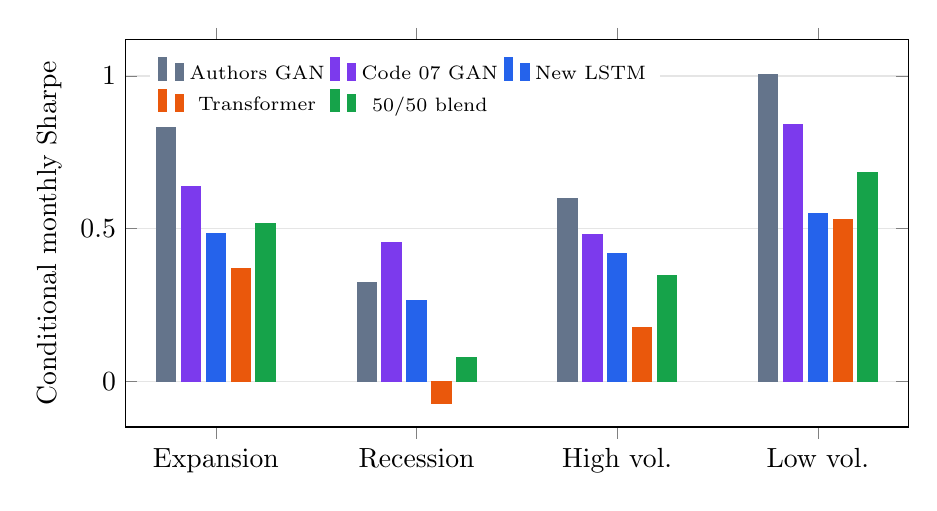
\begin{tikzpicture}
\begin{axis}[width=.95\linewidth,height=6.5cm,ybar,/pgf/bar width=7pt,ymin=-.15,xtick={0,1,2,3},xticklabels={Expansion,Recession,High vol.,Low vol.},ylabel={Conditional monthly Sharpe},enlarge x limits=.15,ymajorgrids,grid style={gray!20},legend style={font=\scriptsize,draw=none},legend columns=3,legend pos=north west]
\addplot[papercolor,fill=papercolor] coordinates {(0.0000,0.841553) (1.0000,0.324262) (2.0000,0.597897) (3.0000,1.003400)};
\addplot[repcolor,fill=repcolor] coordinates {(0.0000,0.636939) (1.0000,0.455282) (2.0000,0.479894) (3.0000,0.841285)};
\addplot[lstmcolor,fill=lstmcolor] coordinates {(0.0000,0.482550) (1.0000,0.263809) (2.0000,0.417369) (3.0000,0.549426)};
\addplot[transcolor,fill=transcolor] coordinates {(0.0000,0.369464) (1.0000,-0.071265) (2.0000,0.177494) (3.0000,0.530793)};
\addplot[blendcolor,fill=blendcolor] coordinates {(0.0000,0.516677) (1.0000,0.076035) (2.0000,0.345000) (3.0000,0.683882)};\legend{Authors GAN,Code 07 GAN,New LSTM,Transformer,50/50 blend}\end{axis}
\end{tikzpicture}\caption{Direct original-versus-replication regime comparison using the authors' supplied monthly series and identical labels. These author-regime statistics are recomputed here; they are not values reported in published Table I. Recession has 26 months.}\label{fig:regimes}\end{figure}


Figure~\ref{fig:regimes} evaluates the historical replication alongside the extensions using the same months and labels. Code 07 monthly Sharpe is 0.637 in expansion, 0.455 in recession, 0.480 in high volatility, and 0.841 in low volatility. It exceeds both new architectures in each of these groups. The blend improves on both new models in expansion and low volatility, but it is weaker than LSTM in recession and high volatility. Diversification benefits are therefore state dependent in the saved sample, rather than uniform.

\clearpage\subsection{Architecture, rolling windows, and regimes together}
Table~\ref{tab:combined} groups rolling statistics by endpoint labels. For 36-month windows ending in recession, Transformer has a slightly higher mean annualized Sharpe than LSTM: 1.409 versus 1.383. For 60-month recession-ending windows, LSTM is higher: 1.893 versus 1.775. This does not contradict the conditional recession-month comparison: trailing windows include returns from earlier economic states.

The fixed blend is strongest in some endpoint groups, especially recession-ending and low-volatility-ending windows, but not in every group. These differences provide descriptive evidence of varying co-movement and relative performance. They do not justify selecting a model by retrospective endpoint labels or selecting favorable windows. Each endpoint partition has been checked to recover the full rolling mean when group means are weighted by their window counts.
\begin{table}[htbp]\centering\small
\caption{Mean annualized rolling Sharpe grouped by regime at the window endpoint; each window includes all of its months.}\label{tab:combined}
\begin{tabular}{lrrrrr}
\toprule
Window & Endpoint regime & Count & LSTM & Transformer & Blend \\
\midrule
36 & Expansion & 239 & 2.058 & 1.473 & 2.191 \\
36 & Recession & 26 & 1.383 & 1.409 & 1.941 \\
36 & High volatility & 117 & 1.642 & 0.893 & 1.489 \\
36 & Low volatility & 148 & 2.268 & 1.921 & 2.701 \\
60 & Expansion & 215 & 1.783 & 1.162 & 1.799 \\
60 & Recession & 26 & 1.893 & 1.775 & 2.469 \\
60 & High volatility & 117 & 1.722 & 1.042 & 1.658 \\
60 & Low volatility & 124 & 1.863 & 1.404 & 2.072 \\
\bottomrule\end{tabular}\end{table}

\begin{figure}[htbp]\centering
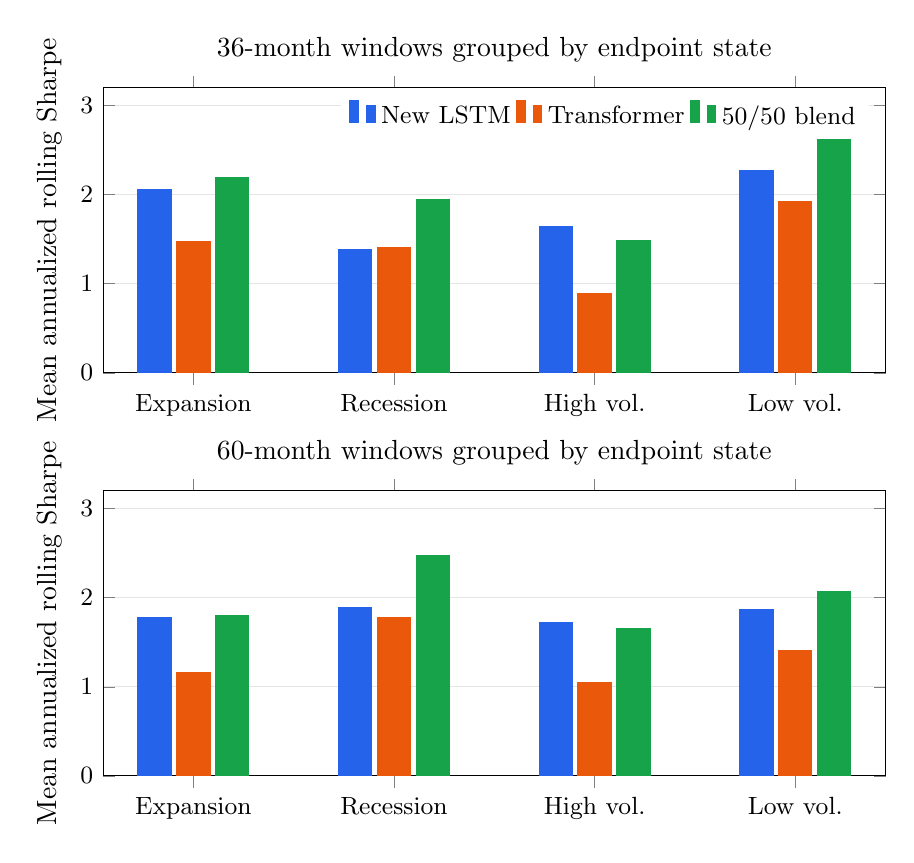
\begin{tikzpicture}
\begin{groupplot}[group style={group size=1 by 2,vertical sep=1.5cm},width=.95\linewidth,height=5.2cm,ybar,/pgf/bar width=12pt,ymin=0,ymax=3.2,xtick={0,1,2,3},xticklabels={Expansion,Recession,High vol.,Low vol.},ylabel={Mean annualized rolling Sharpe},enlarge x limits=.15,ymajorgrids,grid style={gray!20},tick label style={font=\small},legend style={font=\small,draw=none},legend columns=3]
\nextgroupplot[title={36-month windows grouped by endpoint state}]
\addplot[lstmcolor,fill=lstmcolor] coordinates {(0.0000,2.057849) (1.0000,1.382546) (2.0000,1.642119) (3.0000,2.267866)};
\addplot[transcolor,fill=transcolor] coordinates {(0.0000,1.473482) (1.0000,1.409278) (2.0000,0.892840) (3.0000,1.921224)};
\addplot[blendcolor,fill=blendcolor] coordinates {(0.0000,2.190546) (1.0000,1.940987) (2.0000,1.488946) (3.0000,2.701347)};\legend{New LSTM,Transformer,50/50 blend}
\nextgroupplot[title={60-month windows grouped by endpoint state}]
\addplot[lstmcolor,fill=lstmcolor] coordinates {(0.0000,1.783121) (1.0000,1.893402) (2.0000,1.722449) (3.0000,1.863492)};
\addplot[transcolor,fill=transcolor] coordinates {(0.0000,1.162354) (1.0000,1.775244) (2.0000,1.042438) (3.0000,1.404011)};
\addplot[blendcolor,fill=blendcolor] coordinates {(0.0000,1.798995) (1.0000,2.468761) (2.0000,1.658291) (3.0000,2.072191)};\end{groupplot}
\end{tikzpicture}
\caption{Combined architecture, window, and endpoint-regime analysis. Unlike Figure~
ef{fig:regimes}, each statistic uses every return in its trailing window. A recession-ending window may contain expansion returns. Business-cycle and volatility labels are separate partitions.}\label{fig:combined}
\end{figure}

The combined analysis resolves an apparent conflict between Figures~\ref{fig:regimes} and \ref{fig:combined}. Transformer Sharpe is negative when measured only over recession months, but slightly higher than LSTM for 36-month windows ending in a recession. The latter reflects the whole trailing history, not performance earned exclusively during the recession. Reporting both avoids interpreting historical momentum in a trailing statistic as recession protection.

\clearpage\section{Interpretation and limitations}
The experiment does not find an unconditional Sharpe improvement from substituting attention for recurrence under the shortened training budget. This is informative: a more flexible sequence representation is not automatically beneficial when optimization is constrained. However, lower training and validation results do not prove that undertraining is the only explanation. No controlled full-versus-short training ablation has been completed with identical final conventions.

Seed variability measures sensitivity to initialization on a common financial history. Different architectures consume random numbers differently, so same-numbered seed pairs are descriptive matches, not identical random experiments. Similarly, overlapping rolling windows and retrospective regimes do not identify statistical significance. No independent-market confidence interval or formal Sharpe difference test is claimed.

The supplied author GAN series permits direct rolling and regime comparisons; a published scalar Sharpe alone would not permit them. We also do not extend the report to explained variation, cross-sectional pricing errors, characteristic importance, or implementation costs without the necessary model-level inputs. The absence of costs, real-time macro vintages, and a full hyperparameter search limits investment and replication claims. The earlier local GAN is a historical benchmark rather than an otherwise identical full-training control.
\section{Conclusion and next experiment}
The additions produce a linked assessment: architecture establishes the fixed-model comparison, rolling analysis shows temporal variation, conditional regimes show differences across labeled months, and endpoint-regime windows connect the temporal and economic views. The resulting story is more specific than a single Sharpe ranking: LSTM performs better overall under the reduced budget, while relative performance and diversification value vary across time and economic endpoints.

A full-budget, nine-seed experiment for both architectures would be the next direct test of whether the architecture ordering survives more extensive training. Current timing suggests roughly four to five CPU hours for eighteen models, followed by minutes to refresh the evaluation notebooks. That experiment may improve optimization but cannot promise a higher test Sharpe. The present draft reports completed reduced-budget results and makes no numerical prediction for the unfinished full-budget experiment.
\appendix
\section{Reproducible workflow}
Code 07 supplies the historical replication. Code 08 trains the new matched architectures. Code 09 evaluates their fixed returns over rolling windows. Code 10 adds business-cycle and lagged-volatility groups. Code 11 verifies and consolidates model rankings, return/risk, correlations, seed sensitivity, and combined comparisons. Saved CSV tables and notebook outputs are the numerical source of this draft. The consolidated test input contains six models over 300 aligned months; recomputed Sharpes match saved summaries. Combined results additionally verify complete-window counts, constant blend arithmetic, and weighted partition consistency.

The six figures embedded in this document are generated directly from saved CSV results, using inline vector coordinates. The consolidated notebook additionally contains drawdowns, return correlations, seed-versus-ensemble comparisons, rolling distributions, and conditional return/risk diagnostics. The paper and notebook therefore share numerical sources rather than independently transcribed values.
\begin{thebibliography}{9}
\bibitem{cpz} Chen, L., Pelger, M., and Zhu, J. (2021). \emph{Deep Learning in Asset Pricing}. arXiv:1904.00745v6. \url{https://arxiv.org/pdf/1904.00745}. Published Table I benchmarks used here.
\bibitem{code} Authors' training implementation. \emph{Deep\_Learning\_Asset\_Pricing}, audited commit \texttt{6c26b9dad01e76b214ab8f5566c42a29e99677c9}. \url{https://github.com/LouisChen1992/Deep_Learning_Asset_Pricing}.
\bibitem{fred} Federal Reserve Bank of St. Louis. USREC: NBER-based recession indicator. \url{https://fred.stlouisfed.org/series/USREC}. Cached local observations used for descriptive labels.
\end{thebibliography}
\end{document}
